\documentclass{article}

% if you need to pass options to natbib, use, e.g.: \PassOptionsToPackage{numbers, compress}{natbib}
% before loading nips_2016
% to avoid loading the natbib package, add option nonatbib: \usepackage[nonatbib]{nips_2016}

\PassOptionsToPackage{numbers, compress}{natbib}
\usepackage{nips_2016}
% to compile a camera-ready version, add the [final] option, e.g.:
%\usepackage[final]{nips_2016}

\usepackage[utf8]{inputenc} % allow utf-8 input
\usepackage[T1]{fontenc}    % use 8-bit T1 fonts
\usepackage{hyperref}       % hyperlinks
\usepackage{url}            % simple URL typesetting
\usepackage{booktabs}       % professional-quality tables
\usepackage{amsfonts}       % blackboard math symbols
\usepackage{nicefrac}       % compact symbols for 1/2, etc.
\usepackage{microtype}      % microtypography
\usepackage{graphicx}
\usepackage{caption}
\usepackage{subcaption}

\usepackage{amsmath,amsthm,color,graphicx,verbatim,listings,enumitem}
\usepackage[]{algorithm2e}
\graphicspath{{figures/}}

\lstset{
numbers=left, 
numberstyle=\small, 
numbersep=8pt, 
frame = single, 
language=matlab, 
framexleftmargin=20pt}

\newtheorem{lemma}{Lemma}
\newtheorem{theorem}{Theorem}

\title{A Simple Minibatch Acceptance Test for MCMC}

% The \author macro works with any number of authors. There are two commands used to separate the
% names and addresses of multiple authors: \And and \AND.
% Using \And between authors leaves it to LaTeX to determine where to break the lines. Using \AND
% forces a line break at that point. So, if LaTeX puts 3 of 4 authors names on the first line, and
% the last on the second line, try using \AND instead of \And before the third author name.

%%  David S.~Hippocampus\thanks{Use footnote for providing further
%%    information about author (webpage, alternative
%%    address)---\emph{not} for acknowledging funding agencies.} \\
%%  Department of Computer Science\\
%%  Cranberry-Lemon University\\
%%  Pittsburgh, PA 15213 \\
%%  \texttt{hippo@cs.cranberry-lemon.edu} \\


\author{
  Haoyu Chen \\
  Department of Computer Science \\
  University of California, Berkeley \\
  \texttt{haoyuchen@berkeley.edu}
  \And
  Daniel Seita \\
  Department of Computer Science \\
  University of California, Berkeley \\
  \texttt{seita@berkeley.edu}
  \And
  Xinlei Pan \\
  Department of Bioengineering \\
  University of California, Berkeley \\
  \texttt{xinleipan@berkeley.edu}
  \And 
  Biye Jiang \\
  Department of Computer Science \\
  University of California, Berkeley \\
  \texttt{bjiang@berkeley.edu}
  \And
  John Canny \\
  Department of Computer Science \\
  University of California, Berkeley \\
  \texttt{canny@berkeley.edu}
}

\begin{document}
\maketitle

\begin{abstract}
Markov chain Monte Carlo (MCMC) methods have many applications in
machine learning. We are particularly interested in their application
to modeling very large datasets, where it is impractical to
perform Metropolis-Hastings tests on the full data. To do this, we
describe a novel acceptance test which is applied to minibatches of
data. Previous work on minibatch Metropolis-Hastings use adaptive
batch sizes, which may use far more than one minibatch of data and therefore
yield few samples.  Here we describe a simpler test on fixed-sized
minibatches. Instead of adaptive batch sizes, our test requires a
precondition on the variance of the log proposal probability
ratio. Given a measurement of this variance, a minibatch size can be
chosen to support the test in one step, which yields a number of
samples proportional to the batch/minibatch ratio. Alternatively, the
variance condition can be used to adjust the temperature of the
sampling distribution to a ``natural'' value to provide regular
samples at a given minibatch size. The resulting proposal/test is only
slightly more complex than a simple SGD update. In this paper we
derive the test, discuss its implementation, and present several
experiments.
\end{abstract}



\section{Introduction}\label{sec:introduction}

Markov chain Monte Carlo (MCMC) sampling is a powerful method for
computation on intractable distributions. MCMC algorithms propose
samples from a proposal distribution $q$ which is in general different
from the target distribution $p$, and decide whether to accept or
reject them based on an acceptance test. The acceptance test is
usually a Metropolis-Hastings
test~\cite{Metropolis1953,hastings70}. For example, for Bayesian
posterior inference, the posterior distribution $p(\theta \mid x_1,
\ldots, x_N) \propto p(\theta)\prod_{i=1}^np(x_i \mid \theta)$ of
parameter $\theta$ based on conditionally independent data
$\{x_i\}_{i=1}^n$ is the target distribution which one aims to
approximate by sampling $\theta$ values. When $n$ is large, it is
very expensive to compute the exact posterior because the
likelihood must be evaluated on every $x_i$.

Many state-of-the-art machine learning methods, and deep learning in
particular, are based on minibatch updates (such as SGD) to a model.
Minibatch updates produce many improvements to the model for each pass
over the dataset, and have high sample efficiency. They also map very
well onto hardware such as GPUs. In contrast, MCMC methods typically
require calculations over the full dataset to produce a new sample. A
recent result from~\cite{cutting_mh_2014} attempted to bridge the gap
between minibatch optimization and MCMC by proposing an \emph{adaptive
  minibatch} method. Their method uses a subset of the $N$ data points
for the MH test each iteration. However the number of points is not
known a priori, and is adjusted dynamically during every test. This
undermines many of the practical advantages of minibatch calculations: 
GPU kernels work best for certain minibatch sizes, memory blocks
can be reused when minibatch size is fixed, etc. 

In this paper, we develop an alternative minibatch acceptance test for MCMC
methods which uses only one fixed-size minibatch per test. Instead of
dynamically adjusting the batch size, we add a prerequisite for the test
based on the variance of the log acceptance probability. If this
variance is small enough, the test requires only a single step. This
variance changes slowly on typical problems, and we can estimate it
before performing the test. The minibatch variance
decreases as the minibatch size grows, so the variance measurement can be
used to set the minimum minibatch size.

There is another advantage when using our test for Bayesian
posterior inference. As the dataset size grows, the posterior distribution
sharpens and often concentrates to a few sharp peaks. Samples from
this distribution will come from those peaks, and will easily become
stuck in one of them (see Section~\ref{ssec:gaussians}).  The samples are not exploring
the posterior parameter %vspace, and are unlikely to concentrate at a
strong local optimum. They therefore fail to accurately represent a
sample of the posterior because of inadequate search (i.e.,
mixing). We argue that it is much more natural to sample the
distribution at a higher temperature determined by the
minibatch size rather than the dataset size. This temperature is
determined in a natural way by the variance prerequisite for our
test. Starting at a high temperature (small minibatch size) which
mixes easily, one can reduce the temperature (increasing minibatch
size) until one reaches the desired target distribution temperature.
Although this approach also involves changing minibatch size, the
changes increase minibatch size monotonically, and only a few changes
are performed in the course of a sampling session.
Annealing can also be used for MAP and ML estimation because changing temperature preserves
posterior modes. 

To be precise, the contributions of this paper are as follows:

\begin{enumerate}[noitemsep]
    \item We develop a new minibatch acceptance test which satisfies detailed balance.
    \item We compare performance of our new test and the adaptive sampling method.
    \item We experiment using the approach for posterior estimation.
\end{enumerate}




\section{Preliminaries and Related Work}\label{sec:related_work}

In standard MCMC methods~\cite{gilks1996markov,brooks2011handbook} for Bayesian inference with
parameter $\theta$ and conditionally independent data, the goal is to compute the distribution
$p(\theta \mid x_1, \ldots, x_N)$.  To do so, one generates a chain of (correlated) samples
$\theta_1, \ldots, \theta_T$ for large $T$ and approximates $p$ using the sample counts.  Each
iteration $t$ has a current $\theta_t$, and a \emph{proposal distribution} $q(\theta' \mid
\theta_t)$ determines a new candidate $\theta'$. With probability $P_a$, the sample is accepted, so
$\theta_{t+1} = \theta'$. Otherwise, $\theta_{t+1} = \theta_t$. This is done by drawing a uniform
random variable $u \sim {\rm Unif}[0,1]$ and accepting if $u < P_a$. Traditionally, $P_a$ is
\begin{equation}\label{eq:traditional}
P_a = \min\left\{ 1, \frac{f(\theta')q(\theta_t \mid \theta')}{f(\theta_t)q(\theta' \mid \theta_t)}
\right\} = \min\left\{ 1, \frac{p(\theta')\prod_{i=1}^N p(x_i \mid \theta')q(\theta_t \mid
\theta')}{p(\theta_t)\prod_{i=1}^N p(x_i \mid \theta_t)q(\theta' \mid
\theta_t)} \right\},
\end{equation}
where $f(\theta_t)=p(\theta_t \mid x_1,\ldots,x_N)$. The $P_a$ from Equation~\ref{eq:traditional}
satisfies detailed balance, so if one samples long enough, one will arrive at a stationary
distribution matching the posterior, though a burn-in period and/or taking every $n$th sample may be
helpful.

Unfortunately, computing $f$ requires the use of all $N$ training data points. Moreover, it is
difficult to design tests using substantially fewer than $N$ points that also satisfy detailed
balance. To reconcile these competing objectives,~\cite{cutting_mh_2014} proposes an adaptive
minibatch MCMC algorithm which uses a sequential hypothesis test. During each iteration, the
algorithm starts with a small minibatch of data and tests the hypothesis that the sample $\theta'$
should be accepted or rejected based on the likelihood ratio. If the test cannot make a decision
over a certain confidence threshold, then they increase the minibatch size and test again. This
process repeats until a decision.  The downside of this algorithm is the need to keep incrementing
the mini-batch size; in the worst case, all $N$ data points may be needed in a single iteration.  A
similar approach from~\cite{icml2014c1_bardenet14} has slightly more robust theoretical properties,
but comes at the cost of more computational time.

The work of~\cite{conf/uai/MaclaurinA14} presents another minibatch MCMC method which gets the
\emph{exact} posterior, so long as there exists a (cheap) lower bound on the log likelihood for each
data point. Their approach is only a starting point, however, and it can be difficult to derive
these lower bounds in general cases. The extra auxiliary variables they introduce also hurt mixing.

There is a separate line of MCMC work on simulating the physics of a probability distribution. By
viewing random variables as particles in a system, one can apply Hamiltonian Monte Carlo
(HMC)~\cite{mcmc_hamiltonian_2010} methods which generate the best case scenario for proposals: high
quality \emph{and} distant.  HMC methods require a full gradient computation of the posterior, which
means they also face the problem of computing the likelihood at each point. Stochastic versions of
HMC~\cite{sghmc_2014,stochastic_thermostats_2014} use a minibatch of data each iteration but require
controlling the noise from sampling to avoid divergence. Langevin
Dynamics~\cite{langevin_2011,conf/icml/AhnBW12} is a similar approach which does not use the
momentum terms in HMC.  Minibatch SGHMC and Langevin Dynamics are orthogonal to our work and are
other ways of attempting to solve the same problem of MCMC methods on big data. We can combine our
methods with these results, as we demonstrate in Section~\ref{ssec:nets}.

%% Daniel: for a further discussion on the 'Firefly' paper, see this blog post:
%% https://xianblog.wordpress.com/2014/04/02/firefly-monte-carlo/
%% Note: this guy also blogged about our earlier ICLR 2015 paper. He's the third author of the SAME
%% paper, which explains why he knows this stuff.




\section{A New Metropolis-Hastings Test}\label{sec:our_algorithm}

For our new MH test, we use two key values, $\Delta$ and $\Delta'$:
\begin{equation}\label{eq:deltas}
\Delta = \log \left( \frac{p(\theta')  \prod_{i=1}^N p(x_i \mid \theta')  q(\theta_t \mid
\theta')}{p(\theta_t)\prod_{i=1}^N p(x_i \mid \theta_t)  q(\theta' \mid
\theta_t)} \right);\;  \Delta' = \log \left( \frac{p(\theta') (\prod_{i=1}^n p(x_i \mid
\theta'))^{\frac{N}{n}} q(\theta_t \mid \theta')}{p(\theta_t) (\prod_{i=1}^n p(x_i \mid
\theta_t))^{\frac{N}{n}} q(\theta' \mid \theta_t)} \right)
\end{equation}
where $p$ and $q$ have similar definitions as in Equation~\ref{eq:traditional}. Thus, $\Delta$ and
$\Delta'$ are the likelihood ratios in log space. Note that the only difference between $\Delta$ and
$\Delta'$ is that they use $N$ and $n$ data terms $x_i$, respectively, and that the latter uses an
$N/n$ scaling term. We assume $n \ll N$ (so $\Delta'$ is substantially faster to compute) and that
the $n$ data points $x_i$ represent a random minibatch of data.

\subsection{The Full Data Test}\label{ssec:deltas_full}

To motivate the use of $\Delta$, we turn to Lemma~\ref{lem:detailed_balance}.

\begin{lemma}\label{lem:detailed_balance}
Let $\Delta$ be defined as in Equation~\ref{eq:deltas}. Any acceptance function $g$ such that
$g(\Delta) = \exp(\Delta) g(-\Delta )$ satisfies detailed balance. That is, $f(\theta_t)p(\theta'
\mid \theta_t) = f(\theta')p(\theta_t \mid \theta')$, where $p(\theta_y \mid \theta_x)$ is the
probability of jumping from $\theta_x$ to $\theta_y$ in our chain.
\end{lemma}

\begin{proof}
We begin by deriving $p(\theta' \mid \theta_t)$. This is equivalent to the probability of proposing
$\theta'$ and then accepting it, so $p(\theta' \mid \theta_t) = q(\theta' \mid \theta_t)g(\Delta).$
Similarly, $p(\theta_t \mid \theta') = q(\theta_t \mid \theta')g(-\Delta).$ Notice that the
probability of accepting a transition from $\theta'$ to $\theta_t$ is $g(-\Delta)$ because this
inverts the fraction inside the logarithm term of $\Delta$.  By assumption, we can expand $g(\Delta)
= \exp(\Delta)g(-\Delta)$ in $p(\theta' \mid \theta_t)$. Doing this, and combining the result with
the definition of $p(\theta_t \mid \theta')$, we get
\begin{equation}\label{eq:combined}
g(-\Delta) = \frac{p(\theta' \mid \theta_t)}{q(\theta' \mid \theta_t)\exp(\Delta)} = \frac{p(\theta_t \mid \theta')}{q(\theta_t \mid \theta')}.
\end{equation}
Rearranging terms and expanding $\exp(\Delta)$, we have
\begin{equation}\label{eq:rearrange}
\frac{p(\theta' \mid \theta_t) f(\theta_t) q(\theta' \mid \theta_t)}{q(\theta' \mid \theta_t) f(\theta') q(\theta_t \mid \theta')} = \frac{p(\theta_t \mid \theta')}{ q(\theta_t \mid \theta')}.
\end{equation}
Cancellations result in $f(\theta') p(\theta_t \mid \theta') = f(\theta_t) p(\theta' \mid
\theta_t)$. Thus, detailed balance is satisfied.
\end{proof}

As a sanity check, the standard Metropolis-Hastings acceptance function $g(\Delta) = \min\{1,
e^\Delta \} = \min\left\{1, \frac{f(\theta')q(\theta_t \mid \theta')}{f(\theta_t)q(\theta' \mid
\theta_t)}\right\}$ satisfies the condition $g(\Delta) = \exp(\Delta)g(-\Delta)$.

For our MH test, the key is that we use a different $g$, the logistic function: $g(\Delta) =
(1+\exp(-\Delta))^{-1}$. Straightforward arithmetic shows that it satisfies the condition in
Lemma~\ref{lem:detailed_balance}.  The logistic function is nice because we can easily sample from
it using the following procedure. At any iteration with a current parameter $\theta_t$ and a
candidate sample $\theta'$, we can compute $\Delta$. Let $u$ be a uniform random variable $u \sim
{\rm Unif}[0,1]$. We accept $\theta'$ if $g(\Delta) > u$, and reject otherwise. This process is
equivalent to sampling a random variable $X$ with cumulative distribution function $F_X(x) = g(x)$,
and accepting if $\Delta > X$ and rejecting otherwise. We can define $X = g^{-1}(u)$ so that its CDF
is the logistic function, which follows because for arbitrary $X = x$, we have
\[
F_X(x) = {\rm Pr}(X \le x) = {\rm Pr}(g^{-1}(u) \le x) = {\rm Pr}(u \le g(x)) = \int_{0}^{g(x)} 1 dx = g(x),
\]
as the density of $u$ is one. Thus, the criteria to accept the candidate $\theta'$ is equivalent to
whether $\Delta > X$. Moreover, $X$ is symmetric about zero, so the acceptance criteria can also be
expressed as $\Delta + X>0$.

\subsection{The Minibatch Version}\label{ssec:deltas_minibatch}

With large datasets, $\Delta$ is intractable to compute. An intuitive fix is to instead use the
minibatch version $\Delta'$. The following lemma characterizes the distribution of $\Delta'$.

\begin{lemma}\label{lem:gaussian}
If the minibatch data is chosen randomly and sufficiently large, then the distribution of $\Delta'$ is approximately Gaussian.
\end{lemma}

\begin{proof}
By expanding the definition of $\Delta'$ from Equation~\ref{eq:deltas}, we get
\[
\Delta' = \log p(\theta') - \log p(\theta_t) + \log q(\theta_t \mid \theta') - \log q(\theta' \mid \theta_t) +
\frac{N}{n}\sum_{i=1}^n (\log p(x_i\mid \theta') - \log p(x_i\mid \theta_t)).
\]
During a given iteration, $\theta_t$ and $\theta'$ are fixed. Therefore, the randomness in $\Delta'$
comes only from the minibatch. Since the minibatch is chosen randomly, the distribution of
$\sum_{i=1}^n (\log p(x_i\mid \theta') - \log p(x_i\mid \theta_t))$ converges to a Gaussian as $n
\to \infty$ by the Central Limit Theorem.
\end{proof}

% Daniel: I decided to put the figure here, so it's closer to the text that references it.
\begin{figure}[t]
    \centering
    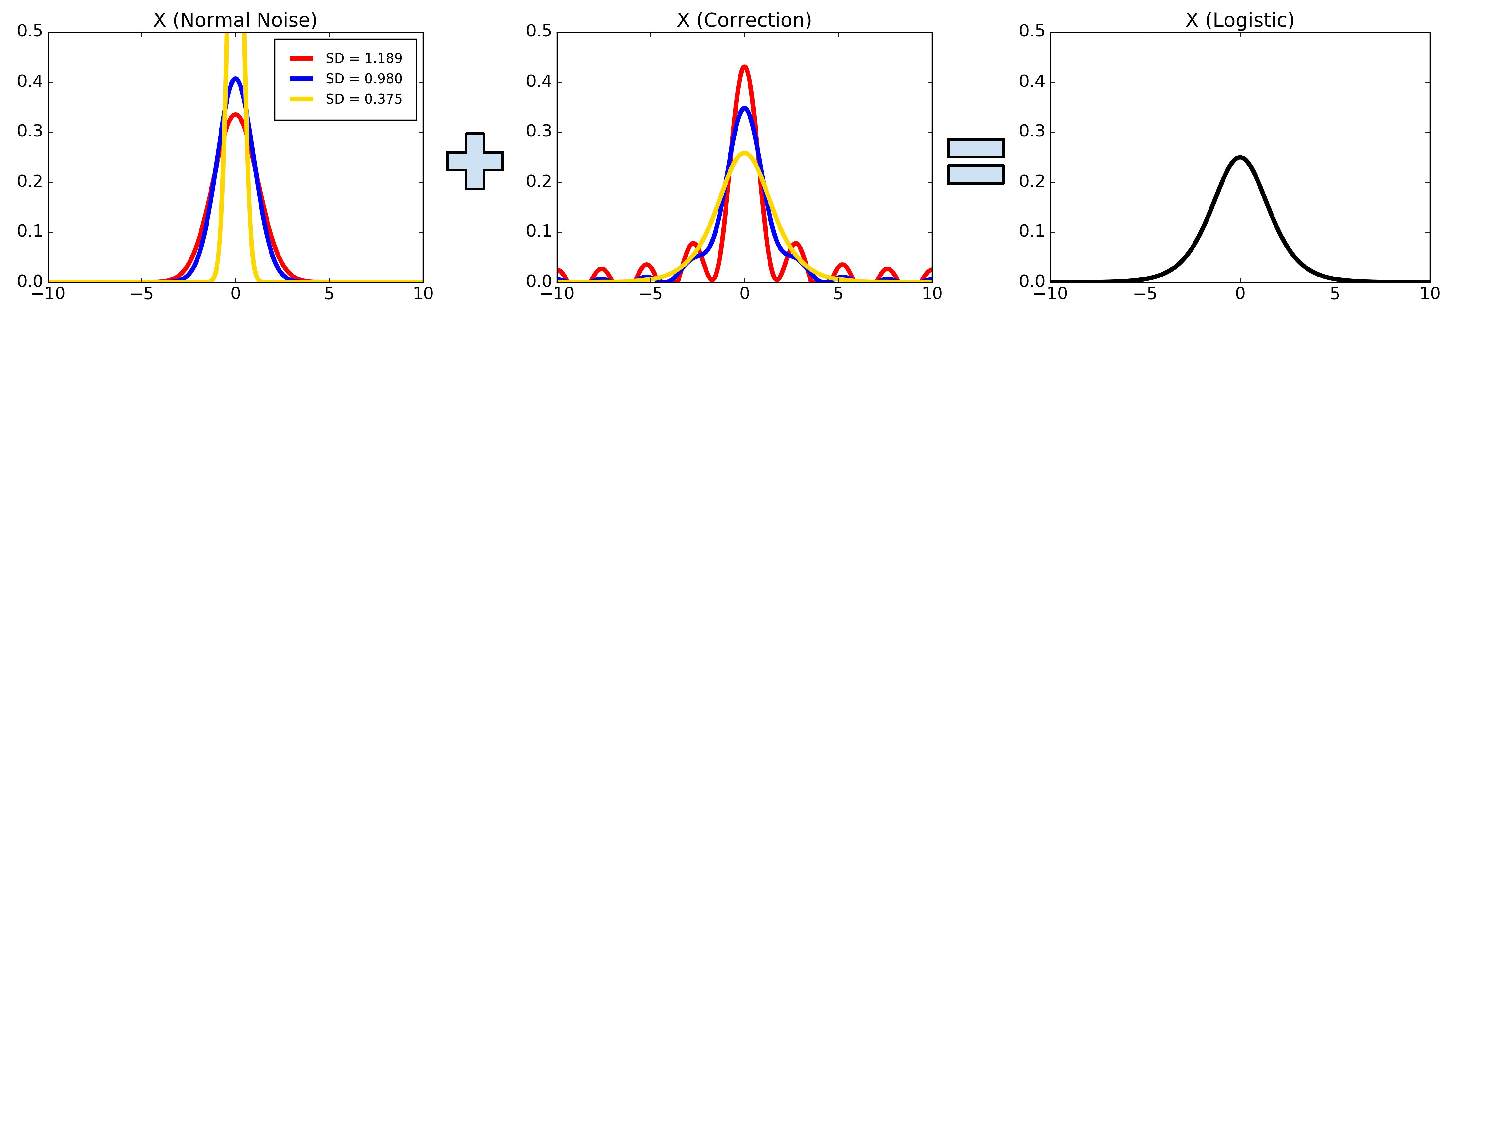
\includegraphics[width=1\textwidth]{mh_convolution_diagram_v2}
    \caption{
    Three examples of $X_{\rm norm}$ and $X_{\rm corr}$ distributions that convolve to form the
    standard logistic distribution. We use three standard deviation values of $X_{\rm norm}$. The
    two red curves convolve to form the logistic, etc. The $y$-axis is capped at 0.5 for
    readability. This figure must be viewed in color.
    }
    \label{fig:deconvolution}
    %\vspace{-10pt}
\end{figure}

From Lemma~\ref{lem:gaussian}, since $\Delta'$ is a noisy approximation of $\Delta$, the
relationship is expressed as
\begin{equation}\label{eq:relationship}
\Delta' = \Delta + \varepsilon, \quad \varepsilon \sim \mathcal{N}(0, \sigma^2),
\end{equation}
for a Gaussian noise term $\varepsilon$.  The extra noise means we can no longer directly perform
the $\Delta + X$ test, so we need to slightly change our acceptance criteria. Our insight is to
decompose $X$ as
\begin{equation}\label{eq:deconvolution}
X = X_{\rm norm}+X_{\rm corr},
\end{equation}
where we assume $X_{\rm norm}$ is a zero-mean Gaussian and $X_{\rm corr}$ is a zero-mean
``correction'' term.  These two add (i.e., their distributions convolve) to form $X$. The criteria
to accept is now
\begin{equation}\label{eq:criteria}
\Delta + X = \Delta + X_{\rm norm} + X_{\rm corr} \approx \Delta' + X_{\rm corr} >0.
\end{equation}
The approximation exists because $X_{\rm norm}$ is an estimate of $\varepsilon$. If $X_{\rm norm}$
is exact, then we get the same MH test with $\Delta'$ as we do with the full data version $\Delta$.

It is important to understand why we use Equations~\ref{eq:deconvolution} and~\ref{eq:criteria}. The
deconvolution process allows us to use $\Delta' + X_{\rm corr}$ as a proxy for $\Delta + X$. It
works because if we know the distribution\footnote{Computing the distributions of $\varepsilon$ and
$X_{\rm norm}$ reduces to finding their standard deviations.} of $\varepsilon$ (from
Equation~\ref{eq:relationship}), then we can pretend that our $\Delta'$ is in fact $\Delta$. To
``insert'' $\varepsilon$ into our test, we deconvolve $X$ so that one of its components, $X_{\rm
norm}$, plays the part of $\varepsilon$. In light of our revised MH test, the previous discussion
raises the question: in an iteration of MCMC with current $\theta_t$ and proposed $\theta'$, how do
we know the distribution of $X_{\rm corr}$? We need the correct distribution to sample the
\emph{values} of $X_{\rm corr}$ appropriately. This procedure consists of two major steps.

\begin{enumerate}[noitemsep]
    \item We first need to estimate the standard deviation of $X_{\rm norm}$. We generate $K$ values
    of $\Delta'$, each using a different random minibatch of $n$ data points, but each using the
    same $\theta_t$ and $\theta'$. In our experiments (see Section~\ref{sec:experiments}), $K$ is
    small, around 5-10, and $n$ is usually a few hundred for the Central Limit Theorem to apply.
    Using these $K$ values, we use the empirical standard deviation ${\rm std}(\Delta')$.

    \item Once we have ${\rm std}(\Delta')$, we can determine the distribution of $X_{\rm corr}$
    from standard deconvolution techniques. These rely on the well-known fact that the Fourier
    transform of a convolution is the product of the Fourier transforms. In practice, we pre-compute
    distributions of $X_{\rm corr}$ for different ${\rm std}(\Delta')$ values to facilitate the
    sampling process.
\end{enumerate}

Algorithm~\ref{alg:our_algorithm} describes our MH test within the MCMC algorithm.

\subsection{Discussions and Practical Considerations of the New MH Test}\label{ssec:discussion}

\SetKwInOut{Input}{Input}
\SetKwInOut{Output}{Output}
\begin{algorithm}[t]
\Input{Number of samples $T$, number of $\Delta'$ estimates $K$, minibatch size $m$, pre-computed $X_{\rm
corr}$ distributions, $\{x_i\}_{i=1}^n$ values from a target distribution, and initial sample $\theta_0$.}
\Output{A chain of $T$ samples $\{\theta_1, \ldots, \theta_T\}$ for either posterior inference or
point estimation.}
\For{$t=\{1, \ldots, T\}$}{
    Propose a candidate $\theta'$ and create an empty list for $\Delta'$ estimates, $d = []$\;
    \For{$k = \{1, \ldots, K\}$}{
        Sample a random minibatch of size $m$ from the complete data\;
        Compute $\Delta'$ from this minibatch (see Equation~\ref{eq:deltas}), and add $\Delta'$ to $d$\;
    }
    Compute ${\rm std}(d)$, the standard deviation estimate of $\Delta'$ from list $d$\;
    \eIf{${\rm std}(d) \ge 1.2$}{
        Skip loop (set $\theta_{t+1}=\theta_t$) and apply variance preconditioning fix (if desired)\;
    }{
        Choose the closest $X_{\rm corr}$ distribution, and sample a value $X_c$ from it\;
        Using another random minibatch of $m$ data points, compute a \emph{new} $\Delta'$ (call it $\Delta_{\rm real}'$)\;
        \eIf{$X_c + \Delta_{\rm real}' > 0$}{
            Accept the candidate, $\theta_{t+1} = \theta'$\;
        }{
            Reject and re-use the old one, $\theta_{t+1} = \theta_t$\;
        }
    }
}
\caption{A description of our MH test within the MCMC algorithm.}
\label{alg:our_algorithm}
%\vspace{-10pt}
\end{algorithm}

\textbf{The Convolution}. Figure~\ref{fig:deconvolution} demonstrates
Equation~\ref{eq:deconvolution} and provides three (color-coded) examples of densities for $X_{\rm
norm}$ and $X_{\rm corr}$. The density of $X$, a logistic random variable with mean $\mu = 0$ and
scale $s=1$, is known, as are the $X_{\rm norm}$ densities for different standard deviations. The
deconvolution provides us with the $X_{\rm corr}$ distributions. Note, however, that as the standard
deviation of $X_{\rm norm}$ increases, the $X_{\rm corr}$ distribution becomes increasingly unstable
and ``bumpier'', because the logistic curve has fatter tails than Gaussians. For this reason, we cap
the standard deviation possibilities of $X_{\rm norm}$ at $\approx 1.2$ in our experiments. In our
experiments, we discretize the possible standard deviations of $X_{\rm norm}$, and we also limit the
densities to consider the range $[-10,10]$ (as shown in Figure~\ref{eq:deconvolution}).

\textbf{Variance Preconditioning}. Returning to the discussion from Section~\ref{sec:introduction},
our test requires a variance check. Equation~\ref{eq:deconvolution} means that the variance of $X$,
which is $\pi^2/3\approx 3.29$ is an upper bound on the variances of $X_{\rm norm}$. Therefore, the
test cannot work if the variance of $X_{\rm norm}$ is too large. Since the standard deviation of $X$
is about $\sqrt{3.29}\approx 1.81$, this bounds ${\rm std}(X_{\rm norm})$ (as well as ${\rm
std}(\Delta')$). From the discussion above, we bound the standard deviation at 1.2 so that $X_{\rm
corr}$ can handle the remaining noise. Recall from Section~\ref{ssec:deltas_minibatch} that we
estimate the ${\rm std}(X_{\rm norm})$ each iteration. If the variance/standard deviation test
fails, then we can (a) skip the iteration, (b) increase the minibatch size, (c) change the proposal
to decrease step sizes, or (d) increase temperature, as we now discuss.

\textbf{Temperature}. One way to satisfy the variance precondition is to increase the temperature of
the target distribution. For a temperature $T>1$, the augmented target distribution would become
\begin{equation}\label{eq:log_temperature}
\log p(\theta \mid x_1,\ldots,x_N) \approx \log p(\theta) + \frac{1}{T}\frac{N}{n} \sum_{i=1}^n\log p(x_i \mid \theta).
\end{equation}
with an extra $1/T$ term augmented. As the temperature increases, the values of $\Delta'$ get
smaller, thus reducing variance. The flatter posterior results in easier mixing of the samples, and
as the samples approach a mode, one can decrease the temperature to sharpen the posterior peaks.




\section{Theoretical Results}\label{sec:theory}

In this section, we explore the convergence properties of our algorithm. Let our true and estimated
acceptance probabilities be $P_a = g(\Delta) = \Pr(\Delta + X > 0)$ and $P_a' = \Pr(\Delta' + X_{\rm
corr} > 0)$. Define our estimate of $X_{\rm norm}$ as $X_{\rm norm}'$, and let $X_{\xi} = X_{\rm
norm} - X_{\rm norm}'$, so that $\Delta' = \Delta + X_{\rm norm} + X_\xi$. We assume the standard derivation of $X_{\rm norm}$ is less than $\pi/\sqrt{3}$, so that we can always apply deconvolution process in Eq~\cite{eq:deconvolution} without using a temperature. We also denote $F_X$ as
the CDF of $X$.  Let the transition kernel of complete data at sampling step $i$ be $P_i$, and let
the transition kernel of minibatch data at sampling step $i$ is $P_i'$. When $P_i$ is apply on one distribution $D$, it generates a new distribution $D'$, we define the transition operation between $P_i$ and $D$ as ``$\circ$''. We show that the distance
of $P_i$ and $P_i'$ is proportional to our estimate error $X_{\xi}$. We also define the stationary
distribution obtained by $P_i$ is $\pi$.  We show the by decreasing the step size, the distribution
of our sampled data converges to $\pi$. We use something called the \emph{total variation distance}
between two kernels, denoted as $\| \cdot \|$.

\begin{lemma}\label{lem:theory1}
If $|X_\xi| < \zeta$ and $\nabla F_X < k$, then $\|P_i-P_i'\| \le 2\zeta k$.
\end{lemma}

\begin{proof}
See Appendix~\ref{app:theory1}.
\end{proof}

Thus, the accuracy of our transition kernel is related to the accuracy of our $X_{\rm norm}$
estimate. We now show that error of our estimation is roughly proportional to the step size of our proposer.

\begin{lemma}\label{lem:theory2}
For one step sampling from $\theta_t$ to $\theta'$, if the jumping step  $|\theta_t - \theta'| <
\epsilon$, and the gradient of the log-likelihood is bounded by a constant factor, i.e. $|\nabla
(\log \Pr(x_i| \theta))| < k$, the variance of $\Delta'$ is bounded by $4\epsilon^2 k^2 m$, where
$m$ is the minibatch size.
\end{lemma}

\begin{proof}
See Appendix~\ref{app:theory2}.
\end{proof}

Since ${\rm Var}(\Delta') < \epsilon^2 k^2 m $, we can assume the maximum value of $X_{\xi}$ is
proportional to the standard deviation of $\Delta'$, i.e. $\epsilon$. Thus, we can assume
$\zeta=\epsilon C$, where $C$ is a constant factor.

\begin{theorem}\label{thm:theory3}
Assume the stationary distribution $\pi$ satisfies $\|T \circ D_0 - \pi\| \leq \eta \|D_0 - \pi\|$,
where $\eta \in [0, 1)$ for all distribution $D_0$. And assume there exists $\rho_t < 1$ such that
$\|P'_i(x, \cdot) - \pi_i'\| \leq 2\rho_i$. We can get $\| P_t' \circ P_{t-1}' \circ \cdots \circ P_1' D_0
- \pi_0 \| \leq \sum_{s=1}^t \{\prod _{u=s+1}^t \rho_u (1-\alpha_u)\} \rho_s \alpha_s + \alpha_t $,
where $\alpha_i = \frac{\epsilon_i C }{1-\eta}$.
\end{theorem}

\begin{proof}
See Appendix~\ref{app:theory3}.
\end{proof}

Theorem~\ref{thm:theory3} indicates that the difference between the target and sampled distributions
consists of two components: $\rho_i$, which is determined by how efficient of $P'_i$, and the
$\alpha_i$s, which are determined by error of our transition kernel. Both are related to the step
size. If step size is large, the $P'_i$ is very efficient, but the error of $P'_i$ increases.
Otherwise, if step size is too small, the $P_i'$ is low efficient, but the error of $P'_i$ is low. 





\section{Experiments}\label{sec:experiments}

In this section, we use three experiments to reveal the benefits of our mini-batch MH testing. For
the first experiment, we illustrate that our mini-batch MH testing can obtain the posterior
distribution which is very close to the ideal one. For the second experiment, we use Logistic
regression to reveal that our mini-batch sampler is much more efficient than adaptive minibatch
approach. The third experiment shows that with the help of temperature, our mini-batch MH testing
can be used to obtain the parameters which are close to MAP. 

\subsection{Mixture of Gaussians}\label{ssec:gaussians}

{\color{blue}
Daniel: TODO Have to show that with more data, the posterior peaks (because it is referenced by the
introduction).
}

We start with a simple mixture of Gaussians, which have tied means:
\[
\theta_1 \sim N(0, \sigma_1^2); \theta_2 \sim N(0, \sigma_2^2); x_i \sim \frac{1}{2}N(\theta_1, \sigma_x^2) + \frac{1}{2} N(\theta_2, \sigma_x^2)
\]
where $\sigma_1^2 = 10, \sigma_2^2 = 1$ and $\sigma_x^2=2$. 200 data points are generated from the
model with $\theta_1 = 0$ and $\theta_2 = 1$. The theoretical posterior distribution can be seen in
Fig.~3a. We use random walk as the proposer. We set the step size 0.1 as a constant. We compare
three scenarios: with our mini-batch MH testing (see Fig.~3b), without our mini-batch MH testing
(see Fig.~3c), and with the standard MH testing (see Fig.~3d). 

\begin{figure}[t]
    \centering
    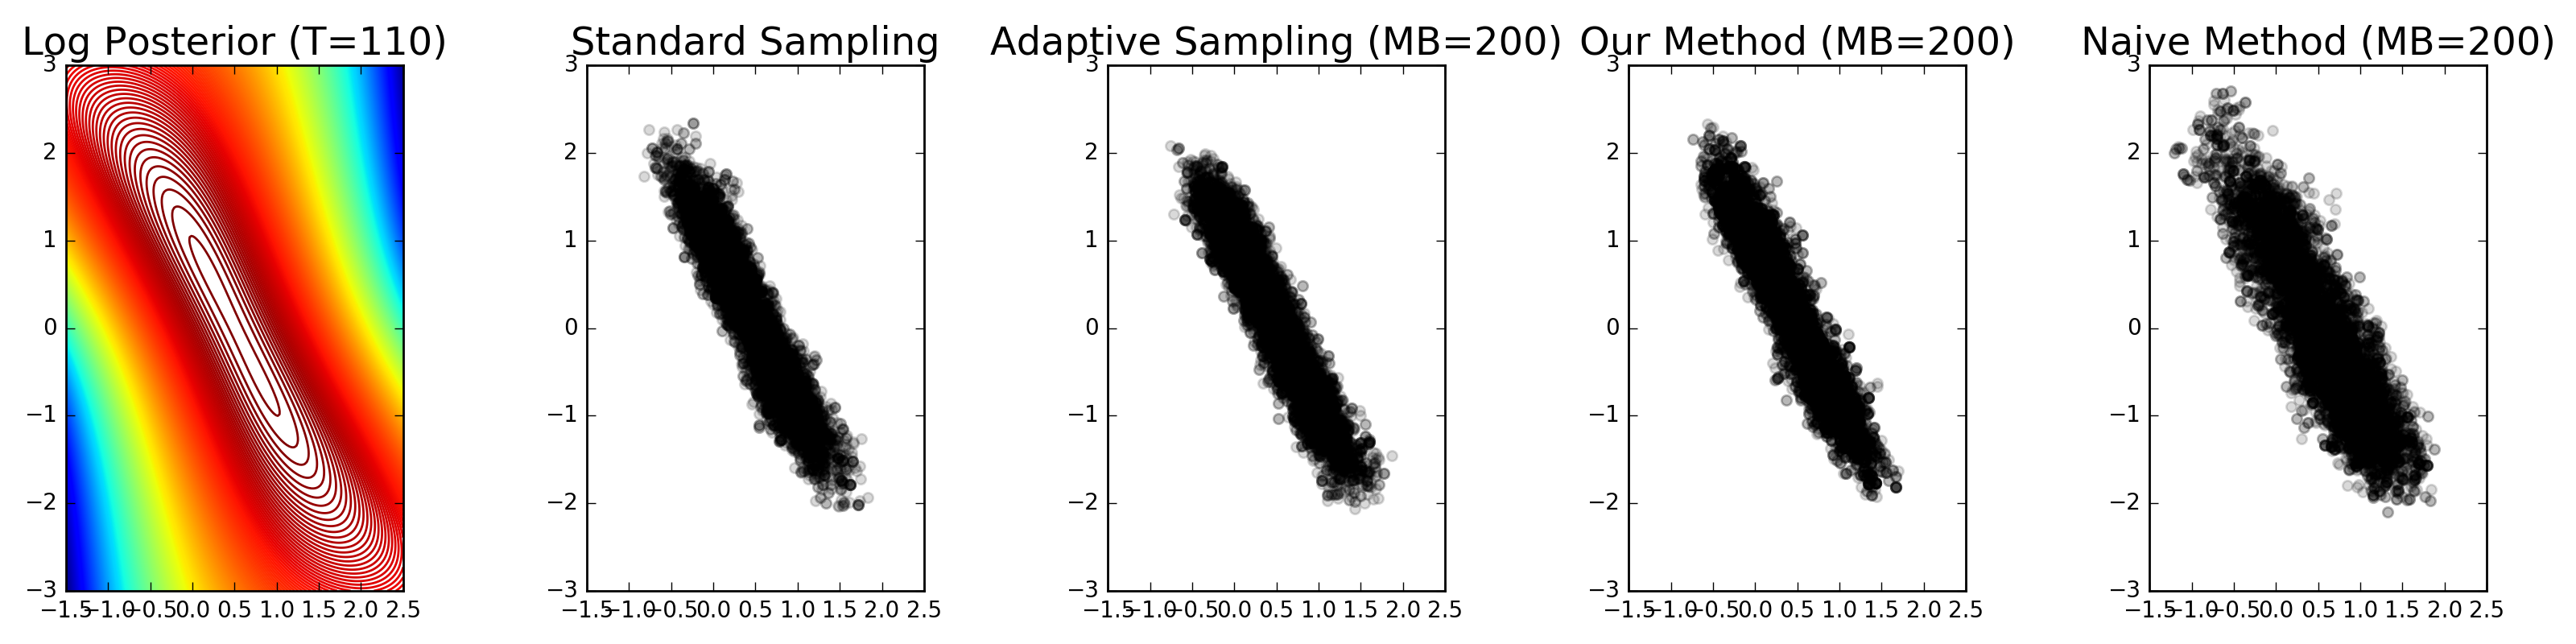
\includegraphics[width=1\linewidth]{cloud_v01.png}
    \caption{
    {\color{blue}
    Daniel: I'll fix the caption later. Basically, true log posterior, standard/adaptive procedures,
    and our method, using MB=200 out of the 10k samples here (also 10k passes over data). All three
    used the same proposal distribution, a RW with a Gaussian of 0.03. Temperature is at 110.
    }
    }
    %\vspace{-10pt}
\end{figure}

\begin{figure}[t]
    \centering
    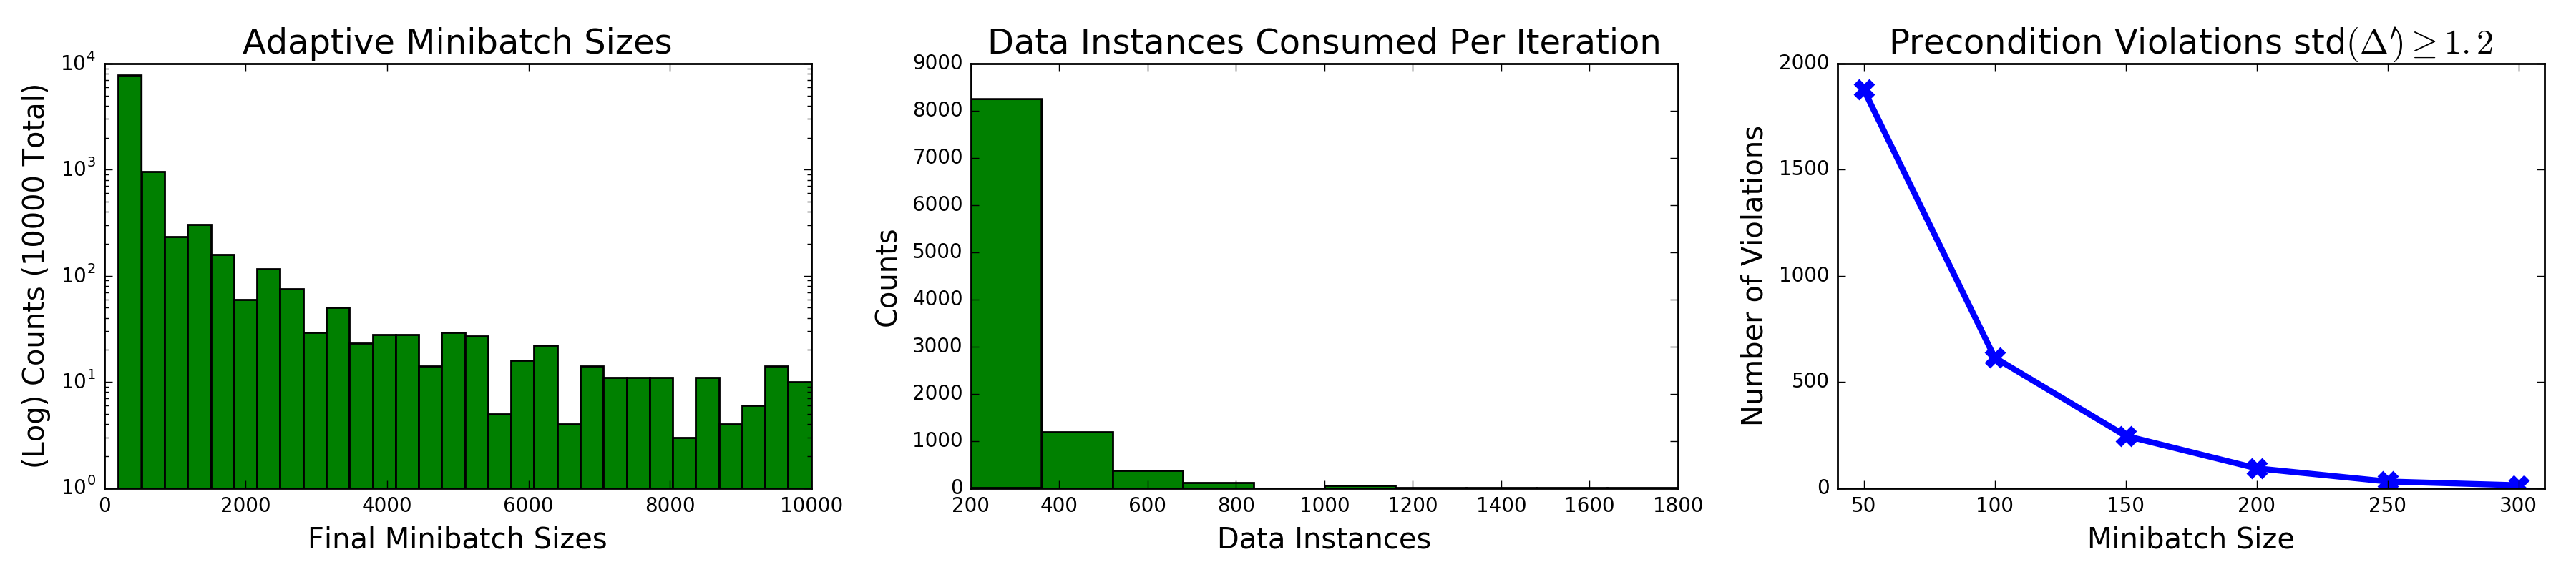
\includegraphics[width=1\linewidth]{adaptive_and_ours_information_v01.png}
    \caption{
    {\color{blue}
    Daniel: I'll fix the caption later. First plot is capped at 1k but the first bin goes up to
    8000. For the SDs, I skipped the ones that didn't satisfy the requirement (a.k.a. repeating the
    previous sample). The third is when I re-ran the experiments but with different minibatches, to
    see how much I would have to repeat. These values were all with one run, though, I might
    consider just taking several (about five?) and doing error bar stuff.
    }
    }
    %\vspace{-10pt}
\end{figure}

From the figures above, we find that with the help of our mini-batch MH testing we can obtain the
sampled distribution which are very close to target one. We feature draw our estimation of standard
derivation of $X_{\rm norm}$ over iterations, see Fig.~3e. We find with even constant step size, the
standard derivation decreases, because the gradient of posterior distribution declines and make the
scale of $\Delta'$ deminished when the sampled point is apporching MAP. Thus, the error our
transition kernel will declines with even constant step size as discribed in Sect.~ 4.

\subsection{Logistic Regression}\label{ssec:logistic}

In this experiment, we use logistic regression to classify the MNIST
dataset~\cite{lecun-mnisthandwrittendigit-2010}. For simplification, we only train the binary
classifier for digits 1 vs 7. The dataset consisted of 12007 training data and 1000 testing data.
Similarly, we use random walk as the proposer. We initilize the temperature as 3000, and decrease it by $t_i = t_0 / (i + 1)^{0.5}$, where $i$ represent the $t^{th}$ iteration. Thus, the standard derivation of $\Delta'$ is smaller than the threshold $\pi/\sqrt{3}$.  We compare our mini-batch MH testing with the
adaptive mini-batch MH testing. Figure 4 shows the log likelihood value and prediction accuracy over
training process. Since the adaptive MH testing method needs to increase the mini-batch size
adaptively, we use the cumulative number of data instance each algorithm consumes as the horizontal
axis. We find our mini-batch MH testing can achieve the similar (or even better log
likelihood/prediction accuracy) with consuming much fewer data points. Thus, we can assert that our
mini-batch MH testing is much more efficient than the adaptive one. 


\begin{figure}[t]
    \centering
    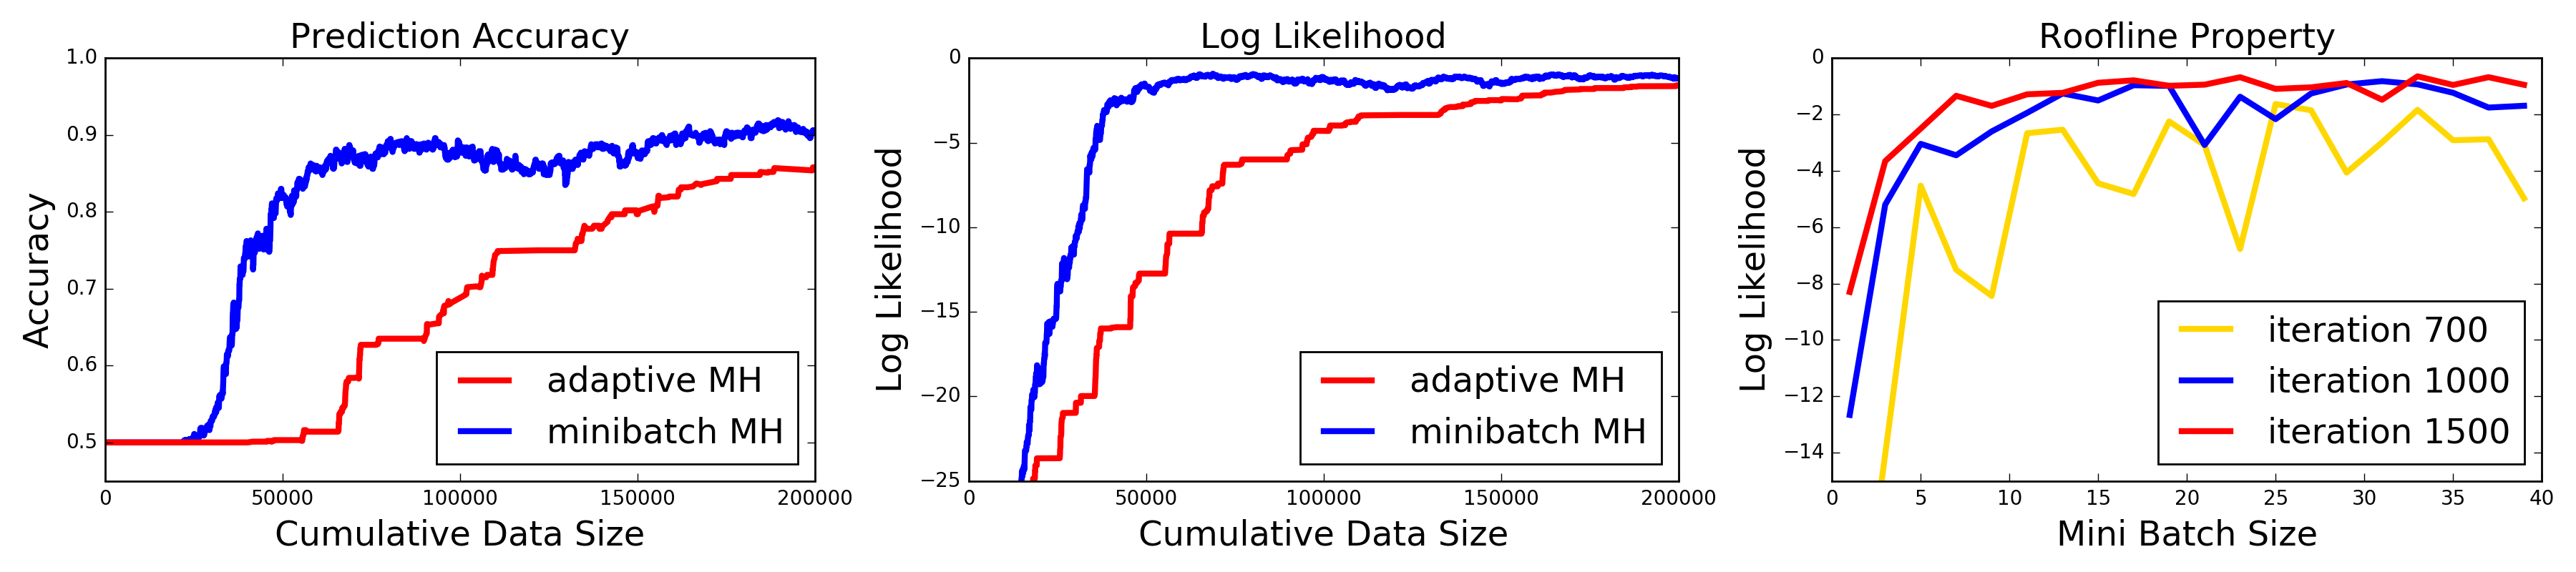
\includegraphics[width=1\linewidth]{exp2.png}
    \caption{Experiment results of Logistic regression}
    %\vspace{-10pt}
\end{figure}

We use this experiment to illustrate another property of our mini-batch MH testing: when the size of
mini-batch increase to a threshold, the accuracy / log likelihood of sampled data at a fix iteration
number will not improve with larger mini-batch size, see Fig.~4c. This is because the variance of
$\Delta'$ decrease with large mini-batch, and the error of our mini-batch MH testing is proportional
to our estimation error of variance of $\Delta'$. When the $var(\Delta')$ decrease to a threshold,
the error of our mini-batch MH testing can be ignored.  

{\color{blue}
Daniel/Haoyu: For additional details, see Appendix~\ref{app:logistic}.
}

\subsection{Neural Network Optimization}\label{ssec:nets}

In this experiment, we apply about mini-batch MH testing with SGHMC (Stochastic Gradient Hamiltonian Monte Carlo, \cite{sghmc_2014}) proposer to sample the parameter instances from a fully connected neural network. We use Higgs data set from University of California Irvine. It is a classification problem to distinguish between a signal process which produces Higgs bosons and a background process which does not. We build a 4 layers neural network to tackle this problem. The first layer is a input layer, the last layer is a softmax layer, the intermediate layers are linear followed by Sigmoid, norm, dropout, starting and ending with linear operation. 

We choose the Adaptive Gradient Descent method ~\cite{adapGrad} as the comparison baseline. Since the frequencies of the features are quite different, we use the same strategy in the Adaptive Gradient to rescale the gradient before apply SGHMC. We implement our system within the open-source BIDMach project~\cite{canny2013bidmach}.  

Figure~5 illustrates our experiment results.  
\begin{figure}[t]
    \centering
    \fbox{\rule[-.5cm]{0cm}{4cm} \rule[-.5cm]{4cm}{0cm}}
    %
\includegraphics[width=0.5\linewidth]{empty}
    \caption{This will hopefully show results for neural networks on BIDMach.}
    %\vspace{-10pt}
\end{figure}




\section{Conclusions}\label{sec:conclusion}

In this paper, we have derived a new MH test for minibatch MCMC methods. We demonstrated how a
simple deconvolution process allows us to use a minibatch approximation to the full data tests. We
experimentally show the benefits our MH test.

Straightforward directions for future work include running additional experiments, with a particular
focus on investigation of the variance precondition.  More elaborate extensions include combining
our results with Hamiltonian Monte Carlo methods, providing a recipe for how to use our algorithm
(following the general framework of~\cite{sgmcmc_2015}), or integrating parallel
MCMC~\cite{conf/uai/AngelinoKWSA14,conf/icml/AhnSW14} concepts into our work.

{\color{blue}
Daniel: TODO, clean this up.
}

\small
\bibliography{nips_2016}
\bibliographystyle{ieeetr}
\normalsize

\clearpage
\appendix

\begin{center}
{\Large Outline of Appendix}
\end{center}

In this appendix, we describe the following topics, with an emphasis on clarity and understanding:

\begin{itemize}[noitemsep]
    \item Some proof details on results in Section~\ref{sec:theory}.
    \item Detailed discussion of the experiment from Section~\ref{ssec:gaussians}.
    \item Detailed discussion of the experiment from Section~\ref{ssec:logistic}.
    \item Detailed discussion of the experiment from Section~\ref{ssec:nets}.
\end{itemize}

\section{Proofs}\label{app:proofs}

\subsection{Proof of Lemma~\ref{lem:theory1}}\label{app:theory1}

We first prove that the difference in our acceptance rates is bounded: $|P_a - P_a'| \leq 2\zeta k$
for some small constant $\zeta > 0$. Given $X_\xi = \xi$ the distance $|P_a - P_a'|$ is:
\begin{align*}
|P_a - P_a'| &= |\Pr(\Delta + X >0) - \Pr(\Delta' + X_{\rm corr} > 0)|\\
& = | \Pr (\Delta + X > 0) - \Pr (\Delta + X_{\rm norm} + \xi + X_{\rm corr} >0) |    \\
&= |\Pr (\Delta + X > 0) -\Pr(\Delta + X + \xi >0)| = |F_X(-\Delta)- F_X(-\Delta - \xi)| \\
&= |\nabla F(-\Delta) \xi + o(\xi^2)| \leq  |\nabla F(-\Delta) \xi| +| o(\xi^2)| \leq 2|\nabla F(-\Delta)| |\xi| \leq 2k \xi,
\end{align*}
where the last line uses Taylor's Theorem ($o(\xi^2)$ represents higher-order terms that have
smaller absolute value) and the Triangle Inequality.  Since $|X_\xi| < \zeta$, $|P_a - P_a'| <
2k\zeta$.

Next, we show the transition kernels at each step are bounded if we use the same proposer, i.e.
$\|P_i - P'_i\| \leq 2k\zeta$. We write $P_i(\theta_t \mid \theta') = P_a(\theta_t, \theta')
q(\theta'\mid \theta_t) + (1-P_a(\theta_t,\theta')) \delta_D(\theta' - \theta_t)$, where $\delta_D$
is the Dirac delta function. The total variation distance between two proposal kernels is
\begin{align*}
\|P_i - P'_i \| &= \int_{\theta'} \left| \int_{\theta_t}((P_a-P_a') q(\theta'|\theta_t) + (1-P_a - 1+P_a') \delta_D(\theta_t -\theta')) d\theta_t  \right| d\theta' \\
& = \int_{\theta'} \left| \int_{\theta_t} (P_a- P_a')(q(\theta'|\theta_t) - \delta_D(\theta_t - \theta')) d\theta_t \right|  d\theta'\\ 
& \leq 2 \zeta k \int_{\theta'} \left| \int_{\theta_t}(q(\theta'|\theta_t) + q(\theta_t|\theta'))  d\theta_t \right| d\theta'= 2 \zeta k,
\end{align*}
as desired.

\subsection{Proof of Lemma~\ref{lem:theory2}}\label{app:theory2}

From Lemma~\ref{lem:gaussian}, only the $\sum_{i=1}^n (\log p(x_i\mid \theta') - \log p(x_i\mid
\theta_t))$ term brings randomness into $\Delta'$. To simplify the subsequent notation, we define
$g_i(\theta) = \log p(x_i\mid \theta)$. Then by Taylor's Theorem:
\[
|g(\theta') - g(\theta_t)| = |\nabla g(\theta_t) (\theta' - \theta_t) + o(\theta' - \theta_t)^2| \leq 2\epsilon k.
\]
Thus, with given the $\theta$, and $\theta'$, the variance of $\Delta'$ can be write as:
\[
{\rm Var}(\Delta') = {\rm Var}\left[\sum_{i=1}^n g_i(\theta') - g_i(\theta_t)\right] \leq
\sum_{i=1}^n  {\rm Var}(g_i(\theta') - g_i(\theta_t)) \leq  4\epsilon^2 m k^2,
\]
as desired.

\subsection{Proof of Theorem~\ref{thm:theory3}}\label{app:theory3}

First, by Theorem 1 in~\cite{cutting_mh_2014}, $\|P_i \circ D_0 - \pi\| \leq \eta \|D_0
- \pi\|$ and $\|P_i-P'_i\| \leq \epsilon_i C$, the norm between the stationary distribution is $\|\pi
- \pi_i'\|\leq \frac{\epsilon_i C}{1-\eta}$.

Second, by Theorem 3.6 in~\cite{yang2013sequential}, we have  $\| P_t' \circ P_{t-1}' \circ \cdots
\circ P_1' D_0 - \pi_t \| \leq \sum_{s=1}^t \{\prod _{u=s+1}^t \rho_u (1-\alpha_u)\} \rho_s
\alpha_s$, where $\alpha = \frac{\epsilon_i C}{1-\eta}$. Thus, we get:
\begin{align*}
 \| P_t' \circ \cdots \circ P_1' D_0 - \pi_0 \| &\leq \|P_t' \circ \cdots \circ P_1' D_0 - \pi_t\| + \|\pi_t - \pi_0\| \\
 &\leq \sum_{s=1}^t \left\{\prod _{u=s+1}^t \rho_u (1-\alpha_u)\right\} \rho_s \alpha_s + \alpha_t,
\end{align*}
as desired.




\section{Gaussian Mixture Experiment Details}\label{app:gaussian}

\subsection{Mathematical Assumptions}

We borrow this example from~\cite{langevin_2011}. Our parameter is a 2-D vector $\theta =
(\theta_1, \theta_2)$, where
\begin{equation}
\theta_1 \sim \mathcal{N}(0, \sigma_1^2) \quad \mbox{ and } \quad \theta_2 \sim \mathcal{N}(0, \sigma_2^2)
\end{equation}
where $\mathcal{N}$ indicates the normal distribution (more generally, the multivariate normal). We
consider the above as our prior. Following~\cite{langevin_2011}, we set $\sigma_1^2 = 10$ and
$\sigma_2^2=1$, so the covariance matrix of $\theta$ is $\Sigma = {\rm diag}(10,1)$. Therefore, the
log prior probability we endow on $\theta$ is
\begin{equation}
\log p(\theta) = \log \left(\frac{1}{2\pi\sqrt{10}}\right) - \frac{1}{2}\theta^T\Sigma^{-1}\theta.
\end{equation}
To generate the data, we use the following Gaussian mixture with tied means:
\begin{equation}\label{eq:x_points}
x_i \sim \frac{1}{2}\mathcal{N}(\theta_1, \sigma_x^2) + \frac{1}{2}\mathcal{N}(\theta_1+\theta_2, \sigma_x^2)
\end{equation}
where, again following~\cite{langevin_2011}, we set $\sigma_x^2 = 2$. This means the log likelihood
of a single data instance is
\begin{equation}
\log p(x_i \mid \theta) = \log\left(\frac{1}{4\sqrt{\pi}}\right) +
\log\left(\exp\left(-\frac{1}{4}(x_i - \theta_1)^2\right) + \exp\left(-\frac{1}{4}(x_i -
(\theta_1+\theta_2))^2\right)\right)
\end{equation}
Here is the problem statement. Given some number of i.i.d. data points $x_1, x_2, \ldots, x_N$
generated according to~(\ref{eq:x_points}), determine the posterior distribution\footnote{Note that,
as is typical with Bayesian analysis, we do not concern ourselves with the denominator of the
original (non-log) posterior.} of $\theta$:
\begin{equation}\label{eq:log_post}
\log p(\theta \mid x_1,\ldots,x_N) = \log p(\theta) + \sum_{i=1}^N\log p(x_i \mid \theta).
\end{equation}
Alternatively, if there are too many data points, we may opt to instead pick a point estimate of
$\theta$, generally the MAP estimate. (If $N$ is extremely large, it will cause the posterior to
peak sharply at its modes, reducing distribution estimates to point estimates.) Note that in many
cases, we will need to take a \emph{minibatch estimate} of~(\ref{eq:log_post}). In that case, the
literature generally uses
\begin{equation}\label{eq:scaling_factor}
\log p(\theta \mid x_1,\ldots,x_N) \approx \log p(\theta) + \frac{N}{n} \sum_{i=1}^n\log p(x_i \mid \theta).
\end{equation}
where we only use $n \ll N$ samples, but we must scale up the likelihood contribution by $N/n$. If we
didn't add this scaling factor, then the contribution of the likelihood terms would be weaker. There
is another thing we need to consider about that, which is the \emph{temperature} of our
distribution. In general, we will want to add $T > 1$ so that our posterior is
$p(\theta)((\prod_{i=1}^n p(x_i\mid \theta))^{N/n})^{1/T}$, resulting in the log
posterior of 
\begin{equation}\label{eq:log_prior_temp}
\log p(\theta \mid x_1,\ldots,x_N) \approx \log p(\theta) + \frac{1}{T}\frac{N}{n} \sum_{i=1}^n\log p(x_i \mid \theta).
\end{equation}
which has the extra $1/T$ to decrease the scale factor.  Equation~(\ref{eq:log_prior_temp}) is what
we will be using for our experiments, because we need to consider warmer distributions.
{\color{blue} Daniel: not totally confident on this but I'll try.}

Finally, recall earlier that we needed to define $\Delta$. In our context, $\Delta$ is:
\begin{align}
\Delta &= \log \left(\frac{f(\theta') q(\theta_t \mid \theta')}{f(\theta_t) q(\theta'\mid \theta_t)} \right) \\
&= \log p(\theta') - \log p(\theta_t) + \sum_{i=1}^N(\log p(x_i \mid \theta') - \log p(x_i \mid \theta_t)) + \log\left(\frac{q(\theta_t \mid \theta')}{q(\theta' \mid \theta_t)}\right).
\end{align}
But again, with \emph{minibatches} of data, we usually do not sum over all $N$ terms and instead sum
over $n$ terms, but with the extra $(1/T)(N/n)$ scaling factor, from
Equation~(\ref{eq:log_prior_temp}). We generally denote that approximation as $\Delta'$ in the paper.

\subsection{Experiment Observations}

\begin{figure}[t]
  \centering
  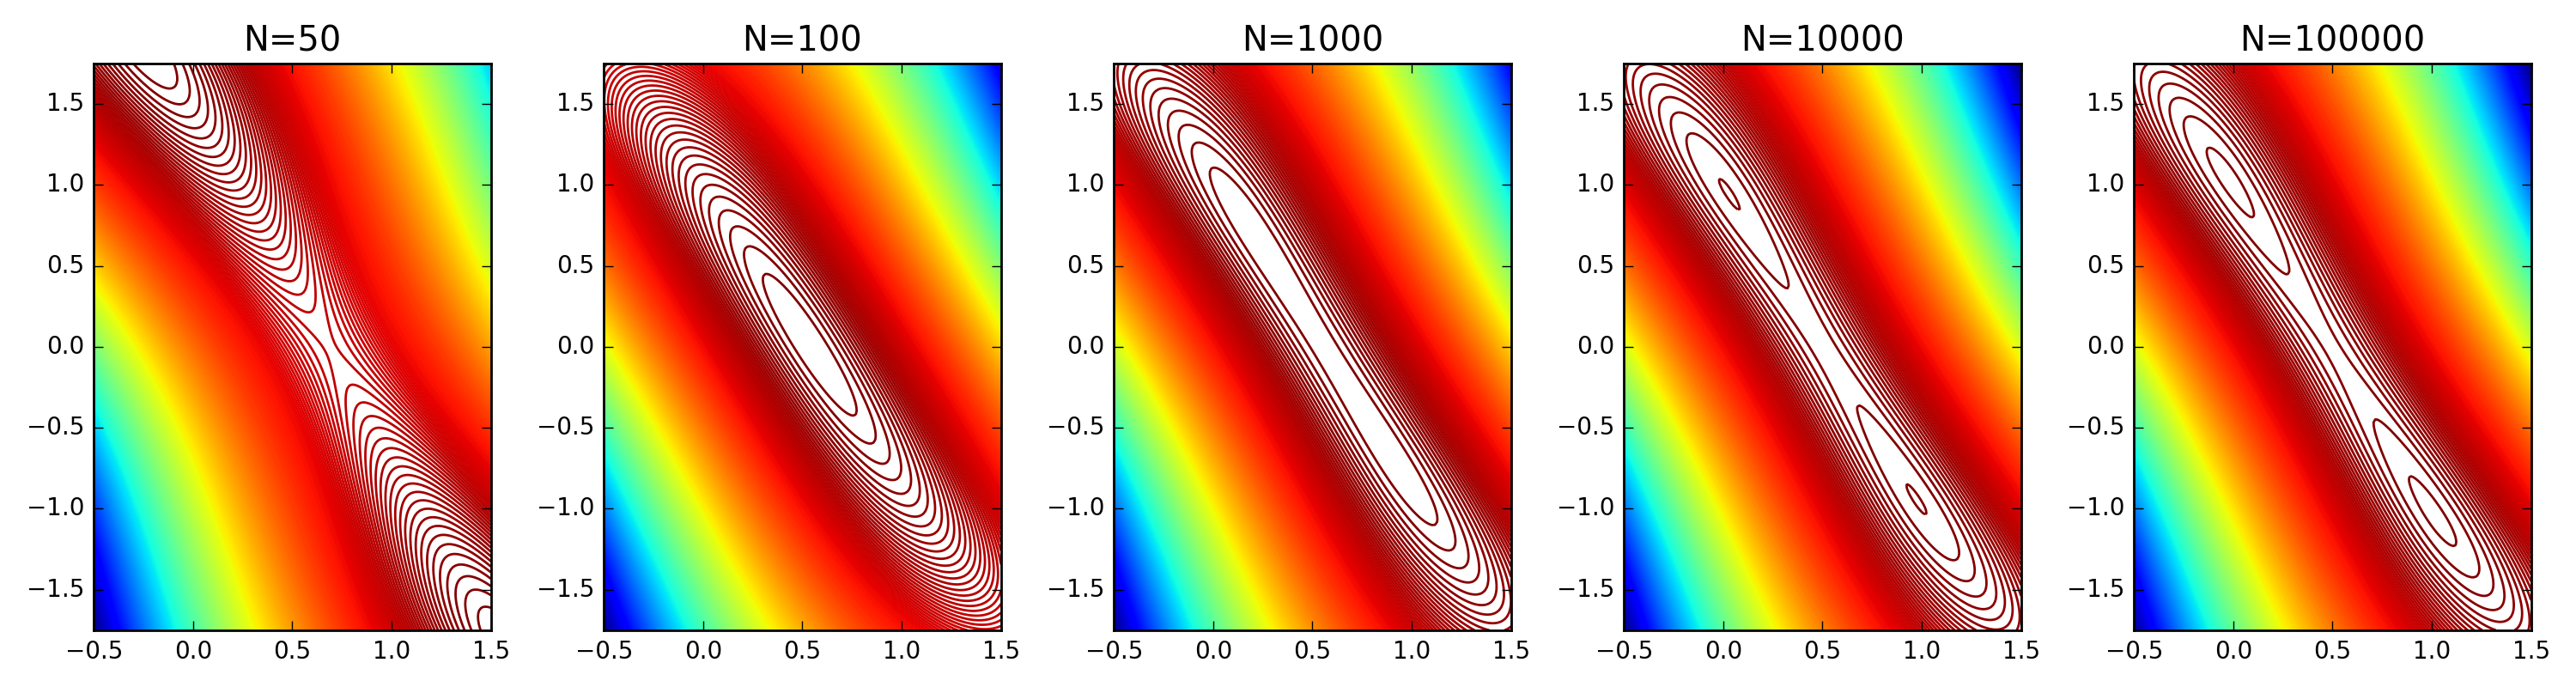
\includegraphics[width=1\linewidth]{contour_v1}
  \caption{The posterior distribution, from 50 to 100k samples, with temperature set at 1.}
  \label{fig:contour1}
\end{figure}
\begin{figure}[t]
  \centering
  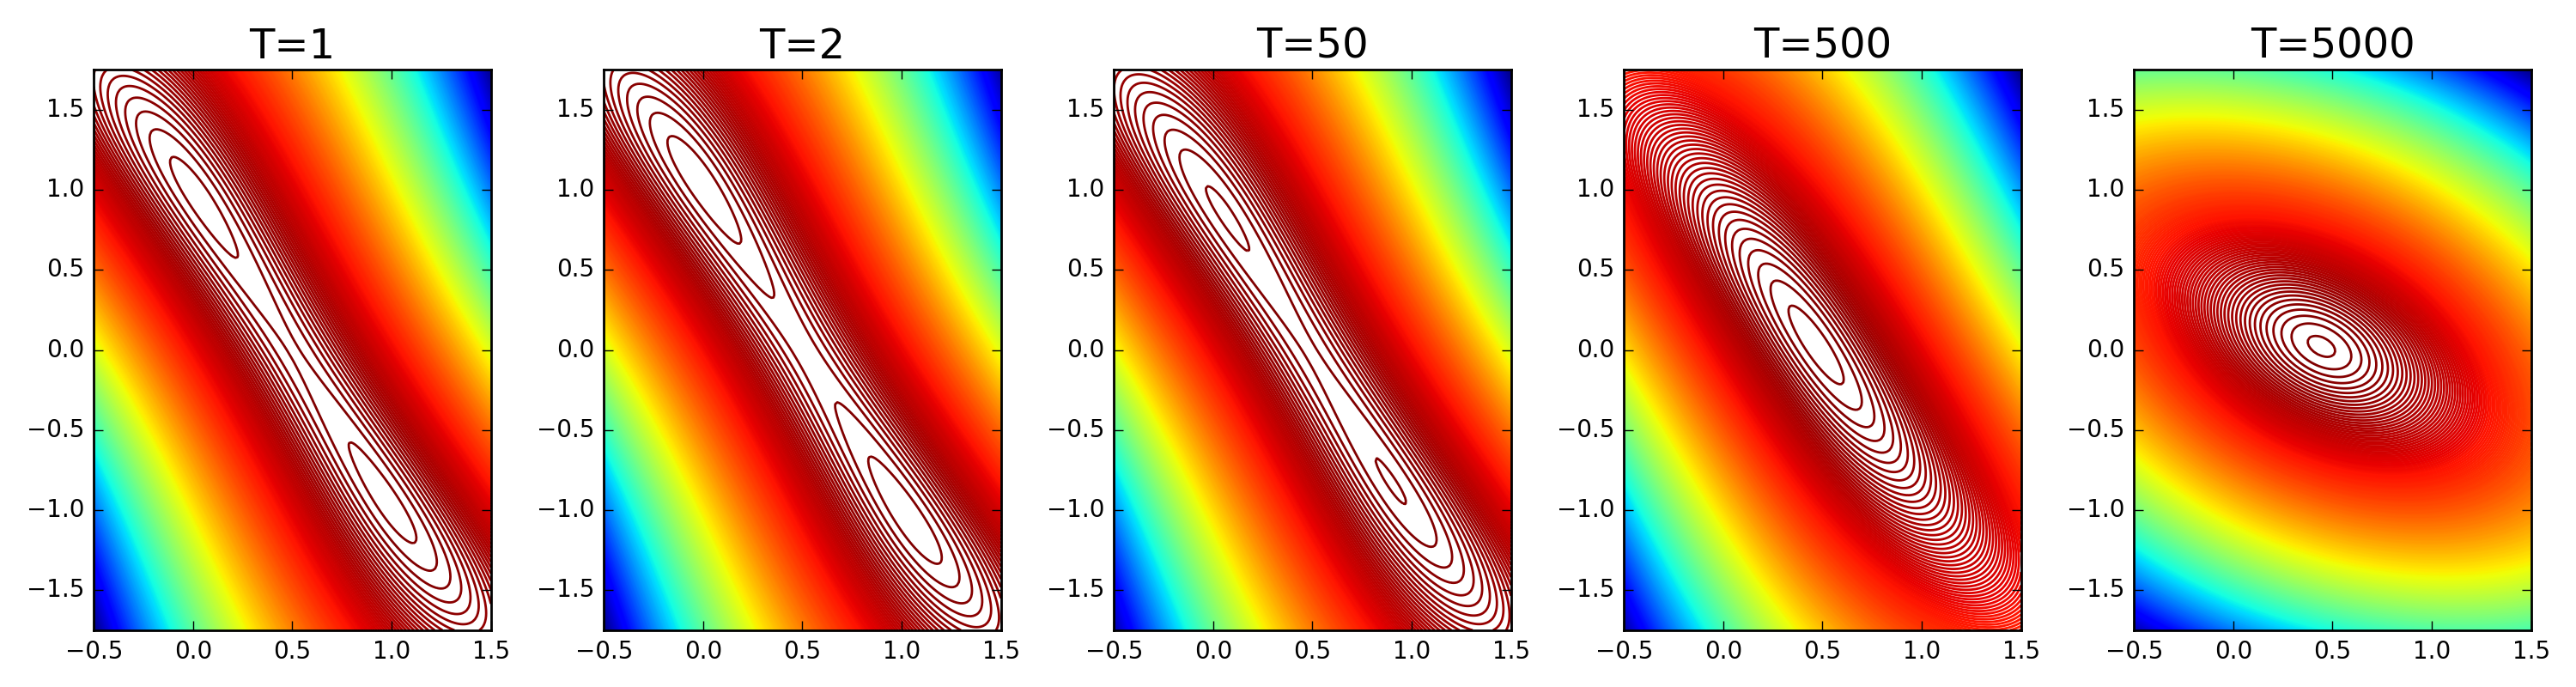
\includegraphics[width=1\linewidth]{contour_v2}
  \caption{The posterior distribution, with $N=10000$ but with temperature $T$ varying.}
  \label{fig:contour2}
\end{figure}

In this experiment, we compare our method with the one from~\cite{cutting_mh_2014}, hereafter called
the ``adaptive sampling approach''. We apply them to the Gaussian Mixture model previously
discussed.

Figure~\ref{fig:contour1} shows simulated contour plots of the posterior based on the $N$ data
points, for varying $N$, with the temperature set at $T=1$. Note that because we're using all $N$
points here, the scale factor $N/n=1$. As $N$ increases, the posterior converges to a multimodal
distribution with modes at $(0,1)$ and $(1,-1)$. 

Figure~\ref{fig:contour2} is similar, except this time we fix the number of samples at $N=10000$,
but show how changing the temperature $T$ affects the distribution. A larger $T$ implies a flatter
posterior, one that (weakly) peaks in between the two true modes.

Our ultimate goal is to either (a) get a posterior distribution that covers the posterior well, or
(b) to get samples that stay trapped at a mode, for a point estimate of $\theta$.  Whether our goal
is (a) or (b) depends on our objectives and the context of the problem (e.g., big data usually
implies (b) is OK even if it would not satisfy the average Bayesian).

For both our method and the adaptive sampling method, we use random walk proposals. (Thus, the term
in $\Delta$ containing the $q$s disappears.)  Random walk proposals are bad, but since the proposal
is poor, good performance can only be obtained with a strong MH test, hence why we can use this as a
reasonable starting benchmark.

We test use the following settings:

\begin{itemize}[noitemsep]
    \item We use $N=10000$ samples of $x_i$.
    \item The covariance of the Gaussian random walk is ${\rm diag}(0.1, 0.1)$.
    \item We use 10000 iterations. One iteration involves one $\theta'$ proposal and a test to
    accept/reject.
    \item The mini-batch size is set at 100, so it is one percent of the total data. For the
    adaptive sampling approach, this is the amount that the minibatch size would keep increasing if
    we needed more precision. Our approach, of courses, keeps the size fixed.
    \item For adaptive sampling, the tolerance for deciding on a test is 0.05. The temperature for
    that is also set at $T=1$ because that algorithm was not designed to deal with temperatures.
    \item For our approach, to get an estimate of the standard deviation of $\Delta'$ (remember,
    $\Delta'$ is a minibatch approximation of $\Delta$) we take five other minibatches (randomly
    selected from the data) and take the standard deviation of those values.
\end{itemize}

For our approach, we run using three different temperature values, $T=1$, $T=10$, and $T=100$.

Figure~\ref{fig:scatter} compares scatter plots of the ``Cutting the MH'' test (hereafter called
``adaptive minibatch'') versus ``Our Method'', where we use three different temperature settings.
There doesn't seem to be too much noticeable difference in our method for the three different
temperature setting values, but our approach is a lot different from the adaptive sampling method
(this is because of rejection rates, more on that later).

\begin{figure}[ht]
  \centering
  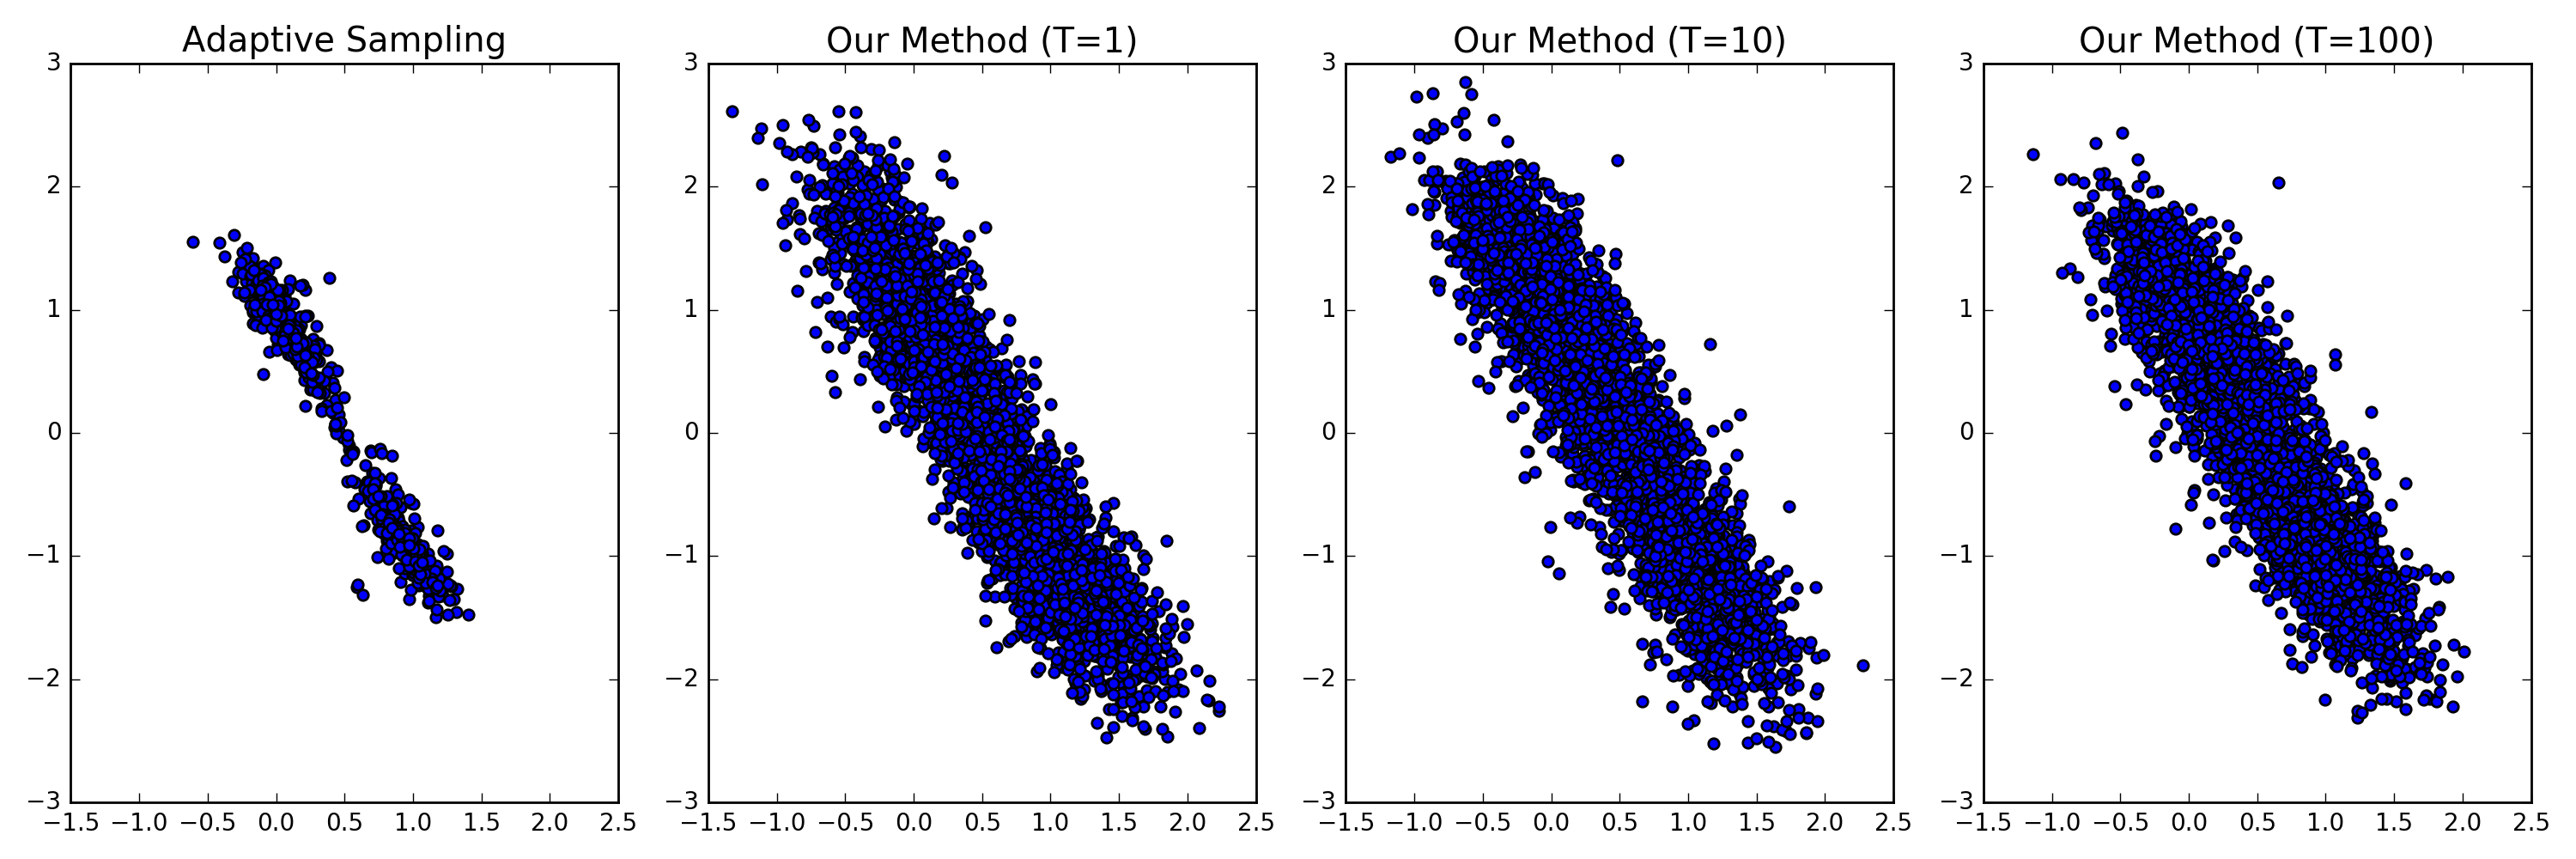
\includegraphics[width=1\linewidth]{scatter_v01}
  \caption{Scatter plots of accepted $\theta$ for (in order) the adaptive sampling approach, and our
  method (temperatures 1, 10, and 100).}
  \label{fig:scatter}
\end{figure}

Before taking a look at our approach, we first examine the adaptive sampling approach. \textbf{That
approach rejected a lot of samples; out of 10000 iterations, it only accepted 773 times}.
Figure~\ref{fig:mb_sizes} describes the histograms of the adaptive minibatch's batch sizes. (Note
that the histogram y-axis values are different.) In many cases, using the initial batch size of 100
sufficed to make an accept/reject decision, but sometimes, this method needed to use the entire 10k
data set. Decreasing the tolerance (from its current 0.05 value) would have required larger
minibatches. Incidentally, it makes sense that the method rejects a lot of samples, because the
random walk proposal usually provides us with poor points.

\begin{figure}[ht]
  \centering
  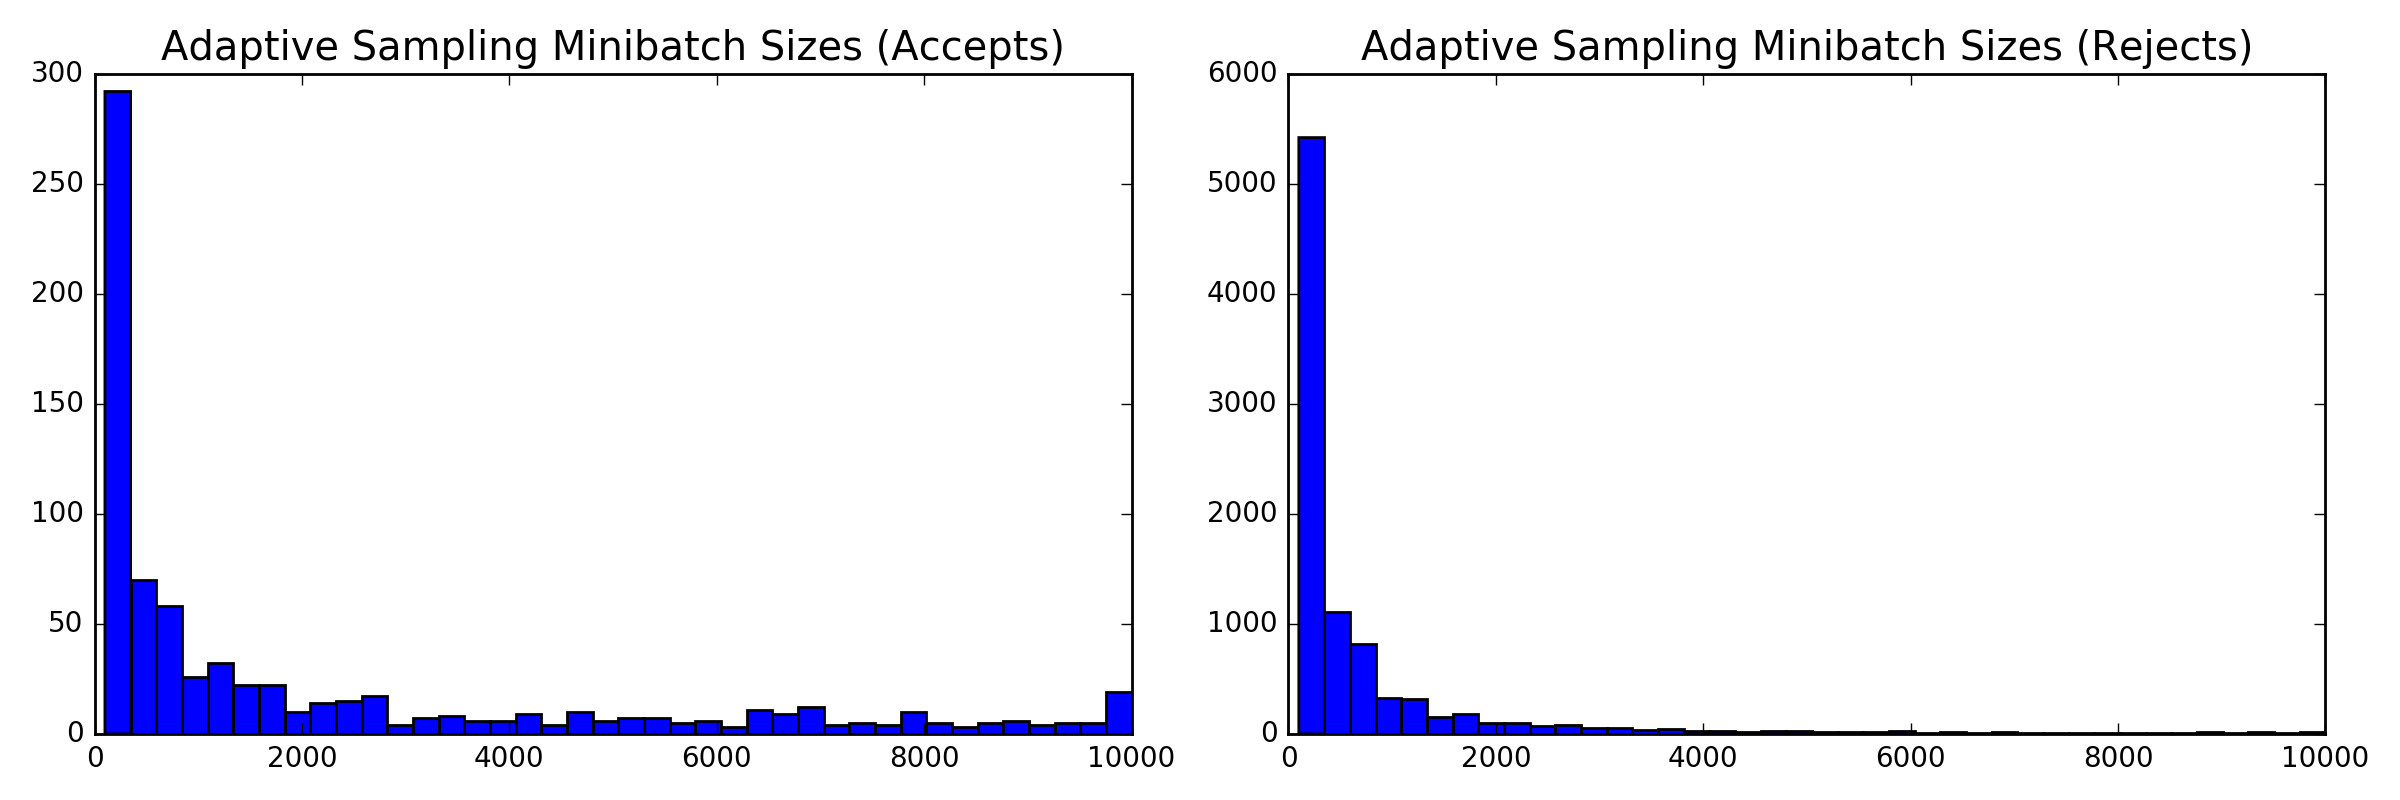
\includegraphics[width=0.75\linewidth]{adaptive_sampling_sizes_v01.png}
  \caption{Minibatch sizes for adaptive sampling when it was accepting or rejecting.}
  \label{fig:mb_sizes}
\end{figure}

Now we analyze our approach in more detail. Our method accepts far more samples than the adaptive
sampling method, \textbf{accepting 3285, 3318, and 3332 out of 10k}, for temperature values 1, 10,
and 100, respectively.

For diagnostics purposes, Figures~\ref{fig:diagnostics1},~\ref{fig:diagnostics2},
and~\ref{fig:diagnostics3} express histograms (for all three temperature runs) of the $\Delta'$,
${\rm std}(\Delta')$, and $X_{\rm corr}$ values, respectively.

There are a few immediate observations. First, increasing the temperature size by a factor of 10
will decrease $\Delta'$ by a factor of 10, which makes sense. That will also directly affect the
standard deviation estimate of $\Delta'$. Our $X_{\rm corr}$ distribution is symmetric about zero,
which is also expected (and it also exhibits a decrease in a factor of 10 for an increase
in temperature).

{\color{blue}
Daniel: One concern I have is that our $\Delta'$ values do not seem to be ``sufficiently negative''. If our
$\Delta'$ values are negative (but large in absolute value) that means our MH test will reject more
often. But then this raises another concern: didn't we say at one point that we \emph{should} be
getting high acceptance rates, around 50 percent (in part because of the shape of the logistic
function)? Doesn't that depend on the quality of the proposal distribution? If our method is
designed to accept a lot regardless of the proposal distribution, I don't see how its performance
can be considered equal to the adaptive sampling approach, or even a standard MH test. In fact, the
best observation I can derive from this is that our approach and the adaptive sampling (or any
standard MH test) will accept the high likelihood cases, but our case will accept the borderline
ones more often.
}

\begin{figure}[ht]
  \centering
  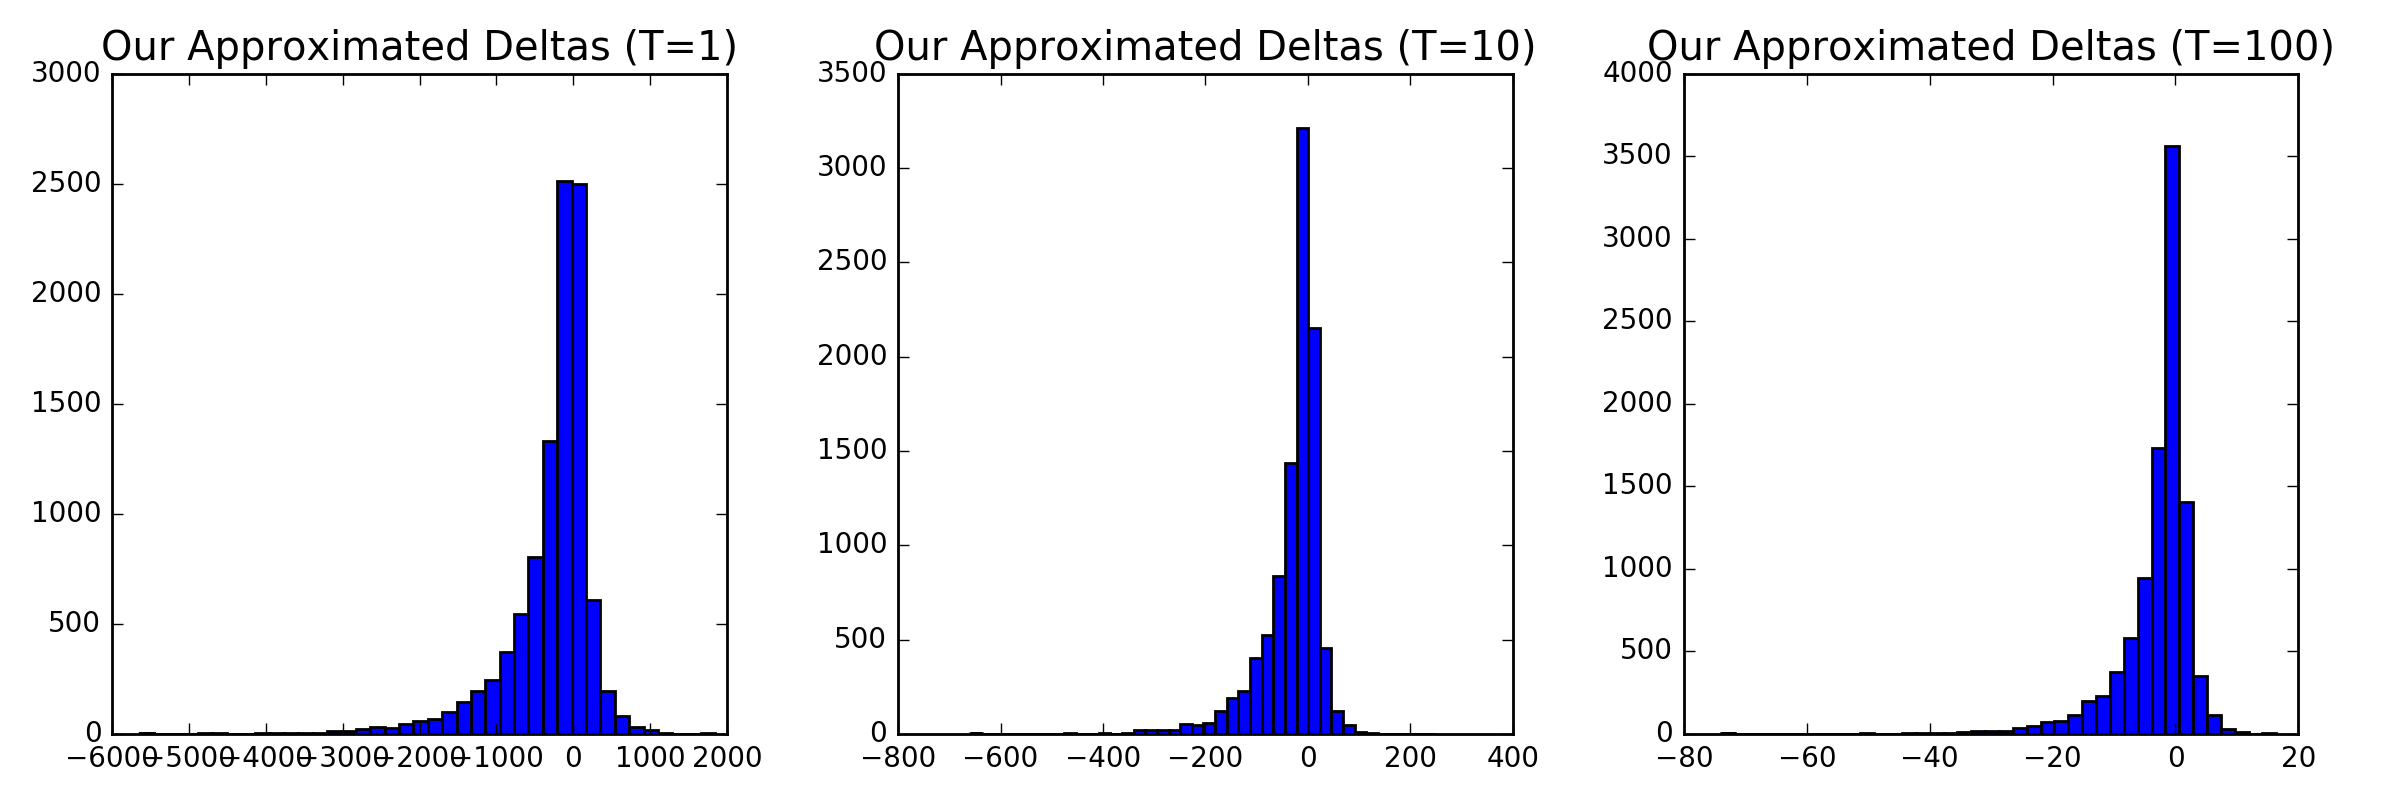
\includegraphics[width=1\linewidth]{our_deltas_v01.png}
  \caption{Our $\Delta'$ values for three different temperature values.}
  \label{fig:diagnostics1}
\end{figure}

\begin{figure}[ht]
  \centering
  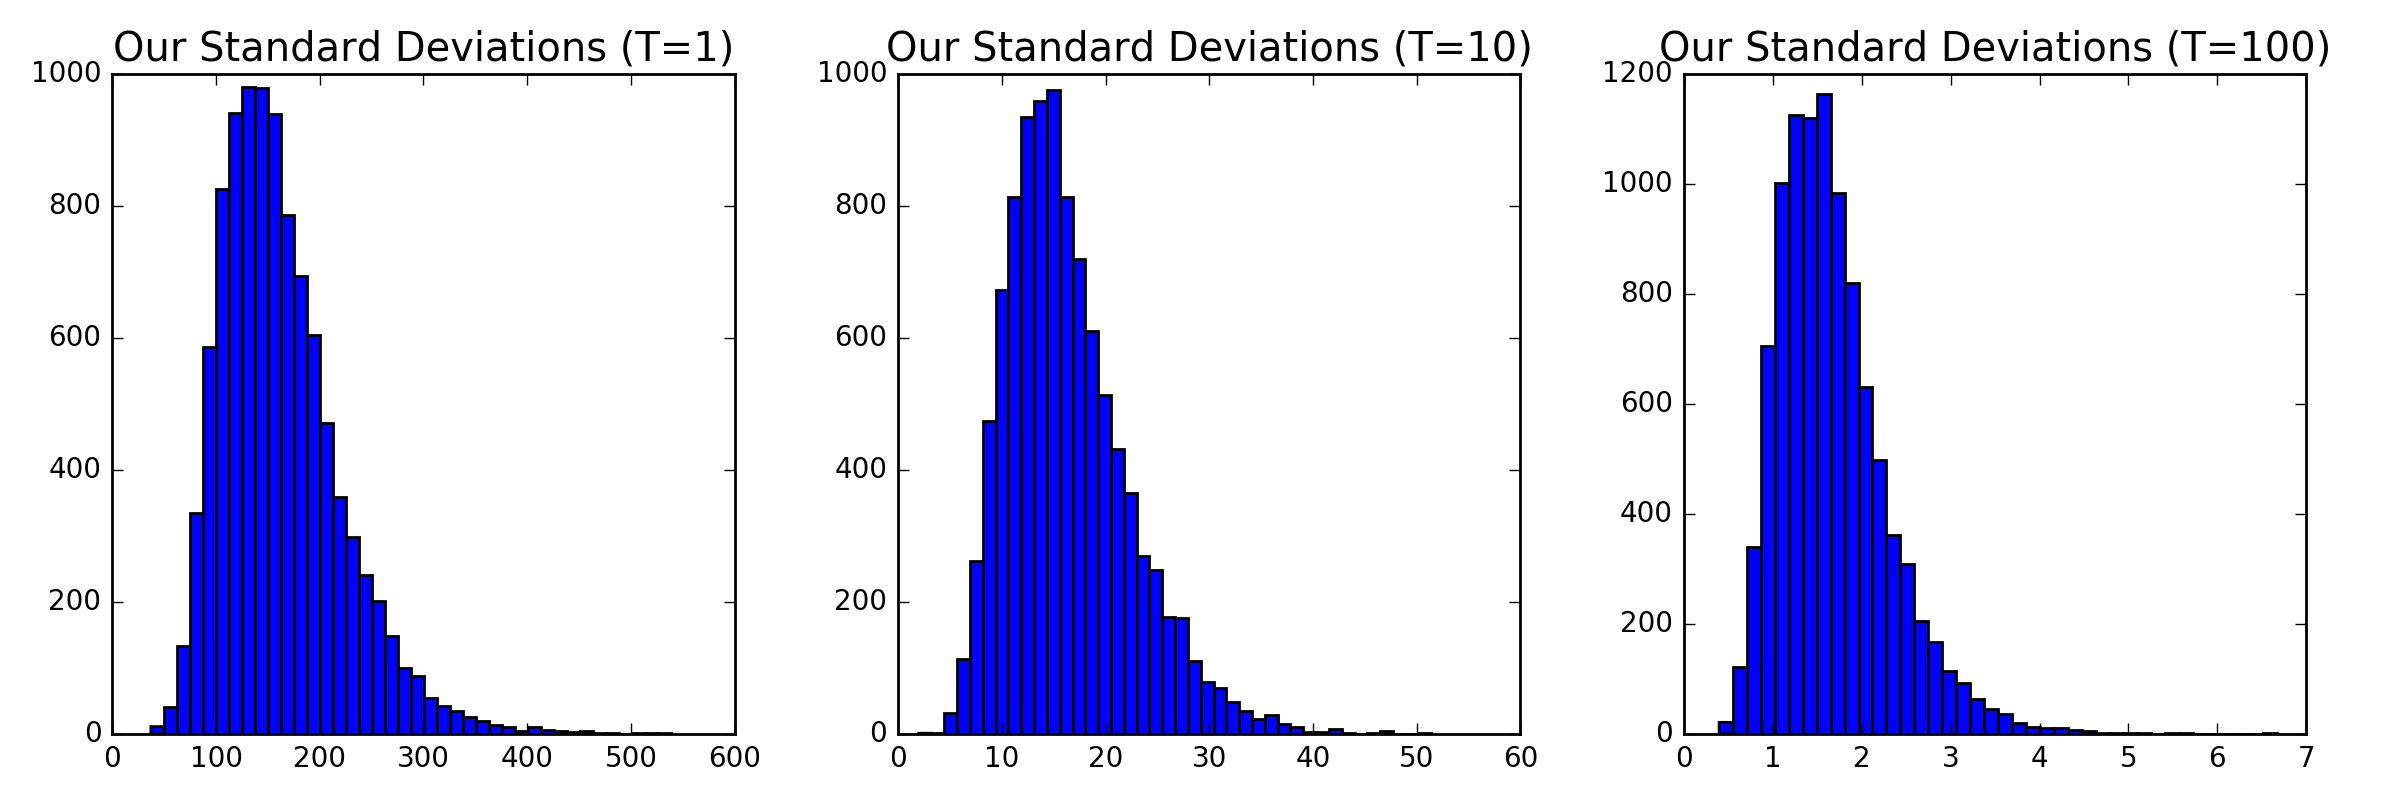
\includegraphics[width=1\linewidth]{our_sds_v01.png}
  \caption{Our ${\rm std}(\Delta')$ values for three different temperature values.}
  \label{fig:diagnostics2}
\end{figure}

\begin{figure}[ht]
  \centering
  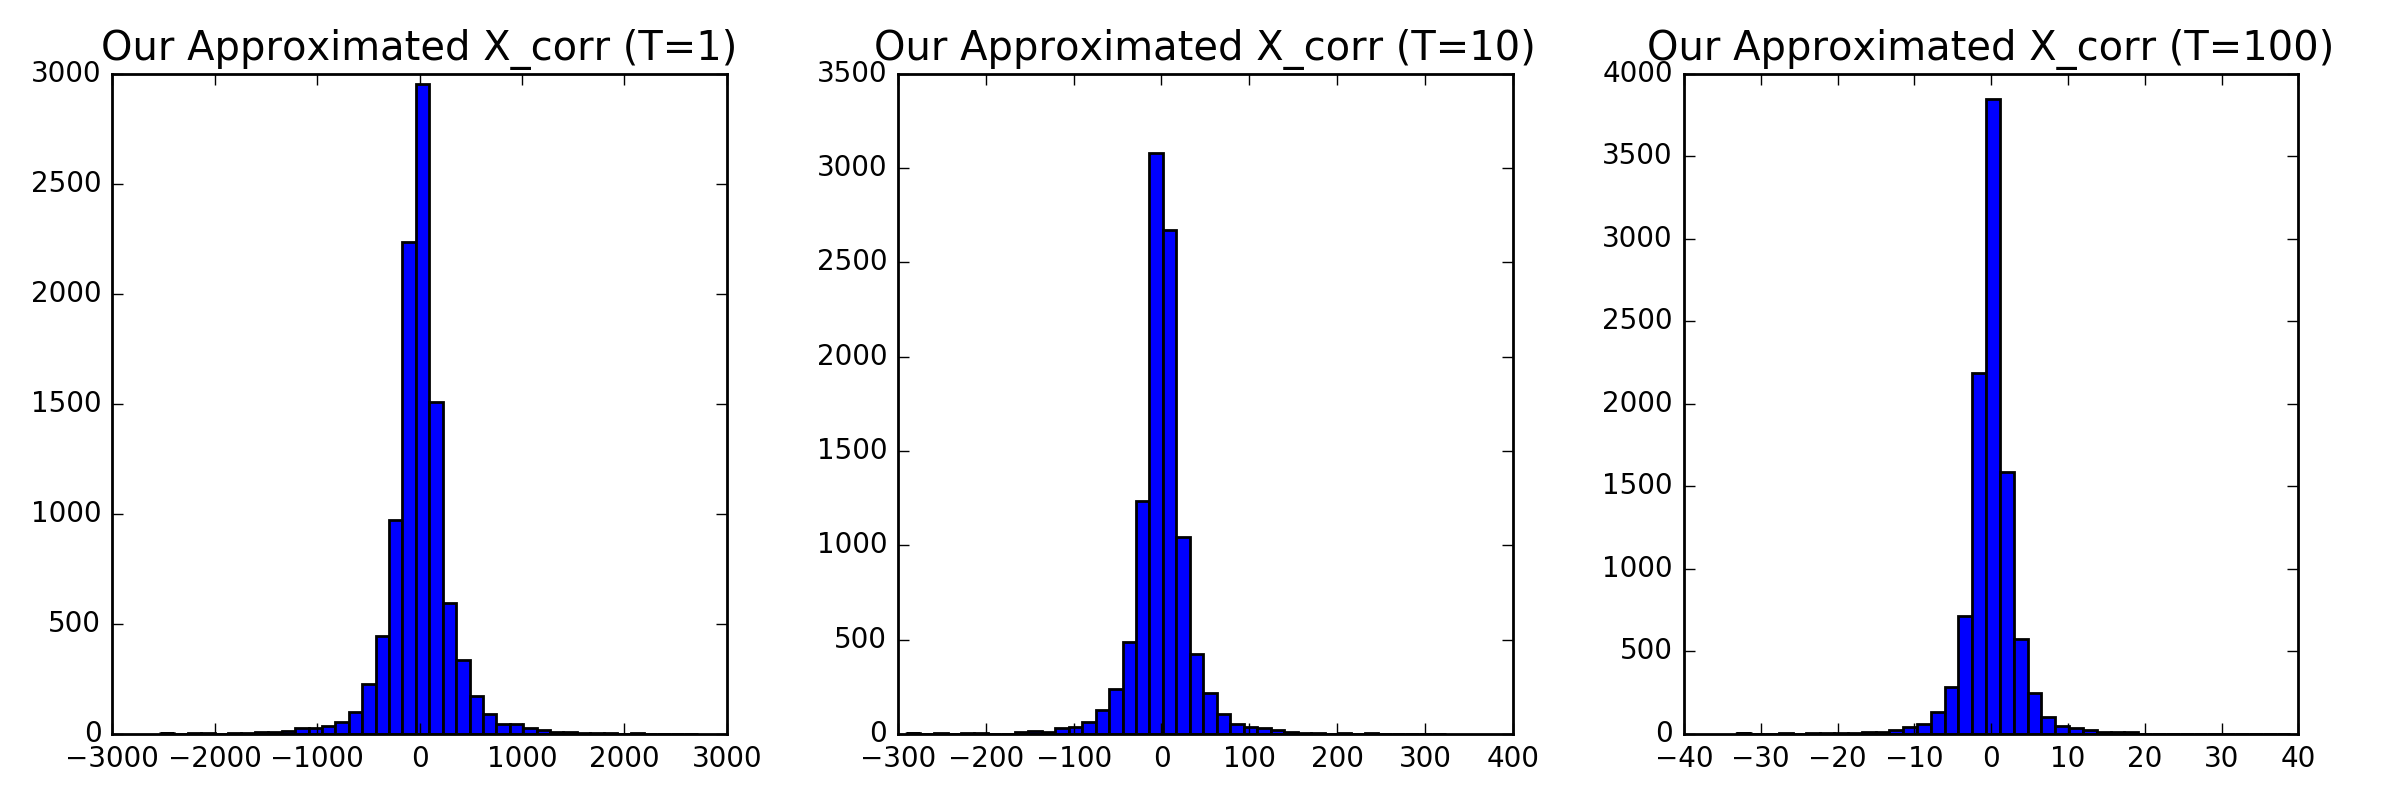
\includegraphics[width=1\linewidth]{our_xcorrs_v01.png}
  \caption{Our $X_{\rm corr}$ values for three different temperature values.}
  \label{fig:diagnostics3}
\end{figure}



\section{Logistic Regression Experiment Details}\label{app:logistic}

We applied our mini-batch Metropolis Hastings algorithm to a Bayesian logistic regression model, comparing with the adaptive sampling method. We tested both our method and the adaptive sampling method using a random walk proposer $q(\theta \mid \theta_t) = N (\theta_t, \sigma^2)$. Since the random walk proposer does not contain any information about the target distribution, it only relies on the Metropolis-Hastings test to converge to the correct distribution. Therefore, random walk proposer is the ideal choice for illustrating our algorithm and comparing with the adaptive sampling method.

\section{Neural Network Experiment Details}\label{app:nnet}

{\color{blue}
Daniel: TODO
}

% Daniel: here are example LaTeX codes for figures and tables if we want to use them.
%\begin{figure}[h]
%  \centering
%  \fbox{\rule[-.5cm]{0cm}{4cm} \rule[-.5cm]{4cm}{0cm}}
%  \caption{Sample figure caption.}
%\end{figure}
%\begin{table}[t]
%  \caption{Sample table title}
%  \label{sample-table}
%  \centering
%  \begin{tabular}{lll}
%    \toprule
%    \multicolumn{2}{c}{Part}                   \\
%    \cmidrule{1-2}
%    Name     & Description     & Size ($\mu$m) \\
%    \midrule
%    Dendrite & Input terminal  & $\sim$100     \\
%    Axon     & Output terminal & $\sim$10      \\
%    Soma     & Cell body       & up to $10^6$  \\
%    \bottomrule
%  \end{tabular}
%\end{table}
%\usepackage[pdftex]{graphicx} ...
%\includegraphics[width=0.8\linewidth]{myfile.pdf}

\end{document}
